\documentclass[handout,compress]{beamer}

\usetheme[block=fill]{metropolis}

\usepackage{graphicx} % Allows including images
\usepackage{amsmath,amsfonts,amsthm,amssymb}
\usepackage{color}
\usepackage{xcolor,cancel}
\usepackage{enumitem}
\setitemize{label=\usebeamerfont*{itemize item}%
	\usebeamercolor[fg]{itemize item}
	\usebeamertemplate{itemize item}}
\definecolor{mDarkBrown}{HTML}{604c38}
\definecolor{mDarkTeal}{HTML}{23373b}
\definecolor{mLightBrown}{HTML}{EB811B}
\definecolor{mMediumBrown}{HTML}{C87A2F}
\definecolor{mygreen}{HTML}{98C2B9}
\definecolor{myyellow}{HTML}{DFD79C}
\definecolor{myblue}{HTML}{8CA7CC}
\definecolor{kern}{HTML}{8CC2B7}


\usepackage{float}
\usepackage{framed}
\usepackage{epsfig}
\usepackage{graphicx}
\usepackage{subcaption}
\usepackage{ulem}
\usepackage{hhline}
\usepackage{multirow}
\usepackage{comment}   
\usepackage{bbm}
\usepackage{tikz}   
\def\Put(#1,#2)#3{\leavevmode\makebox(0,0){\put(#1,#2){#3}}}
\newcommand*\mystrut[1]{\vrule width0pt height0pt depth#1\relax}
\newcommand{\eqdef}{\mathbin{\stackrel{\rm def}{=}}}


\newcommand{\bs}[1]{\boldsymbol{#1}}
\newcommand{\bv}[1]{\mathbf{#1}}
\newcommand{\R}{\mathbb{R}}
\newcommand{\E}{\mathbb{E}}
\newcommand{\blue}[1]{\textcolor{blue}{#1}}

\DeclareMathOperator*{\argmin}{arg\,min}
\DeclareMathOperator*{\argmax}{arg\,max}
\DeclareMathOperator{\nnz}{nnz}
\DeclareMathOperator{\Var}{Var}
\DeclareMathOperator{\sinc}{sinc}
\DeclareMathOperator{\mv}{mv}
\DeclareMathOperator{\sgn}{sgn}
\DeclareMathOperator{\step}{step}
\DeclareMathOperator{\gap}{gap}
\DeclareMathOperator{\poly}{poly}
\DeclareMathOperator{\tr}{tr}
\DeclareMathOperator{\orth}{orth}
\newcommand{\norm}[1]{\|#1\|}
\captionsetup[subfigure]{labelformat=empty}
\captionsetup[figure]{labelformat=empty}
\DeclareMathOperator*{\lmin}{\lambda_{min}}
\DeclareMathOperator*{\lmax}{\lambda_{max}}

\newcommand{\specialcell}[2][c]{%
  \begin{tabular}[#1]{@{}c@{}}#2\end{tabular}}
\newcommand{\specialcellleft}[2][c]{%
\begin{tabular}[#1]{@{}l@{}}#2\end{tabular}
}

\usepackage{tabstackengine}
\stackMath


%----------------------------------------------------------------------------------------
%	TITLE PAGE
%----------------------------------------------------------------------------------------

\title{CS-GY 6763: Lecture 2 \\ Chebyshev's Inequality, Union Bound, Exponential Tail Bounds}
\author{NYU Tandon School of Engineering, Prof. Christopher Musco}
\date{}

\begin{document}

\begin{frame}
	\titlepage 
\end{frame}

\metroset{titleformat=smallcaps}

\begin{comment}
\end{comment}

\begin{frame}
	\frametitle{note on mathematical proofs}
	\small
	It can be hard to know how formal to be. We will try to provide feedback on first problem set for anyone who is either too rigorous or too loose. It's a learning process.
	
	\textbf{Things that are generally fine:}
	\begin{itemize}
		\item Can assume input size $n$ is $> C$ for some constant $c$. E.g. $n > 2, n> 10$.
		\item Similarly can assume $\epsilon < c$ for constant $c$. E.g. $\epsilon < .1$, $\epsilon < .01$.
		\item If I write $O(z)$, you are free to choose the constant. E.g., it's fine if your analysis of CountSketch only works for tables of size $1000\cdot m$. 
		\item Derivatives, integrals, etc. can be taken from e.g. WolframAlpha without working through steps.
		\item Basic inequalities can be used {without proof}, as long as you verify numerically. Don't need to include plot on problem set.
	\end{itemize}
\end{frame}

\begin{frame}
	\frametitle{example inequality}
	\begin{align*}
		1+\epsilon \leq \frac{1}{1-\epsilon} \leq 1+ 2\epsilon \text{ for } \epsilon \in [0,.5].
	\end{align*}
\textbf{Proof by plotting:}
\begin{center}
	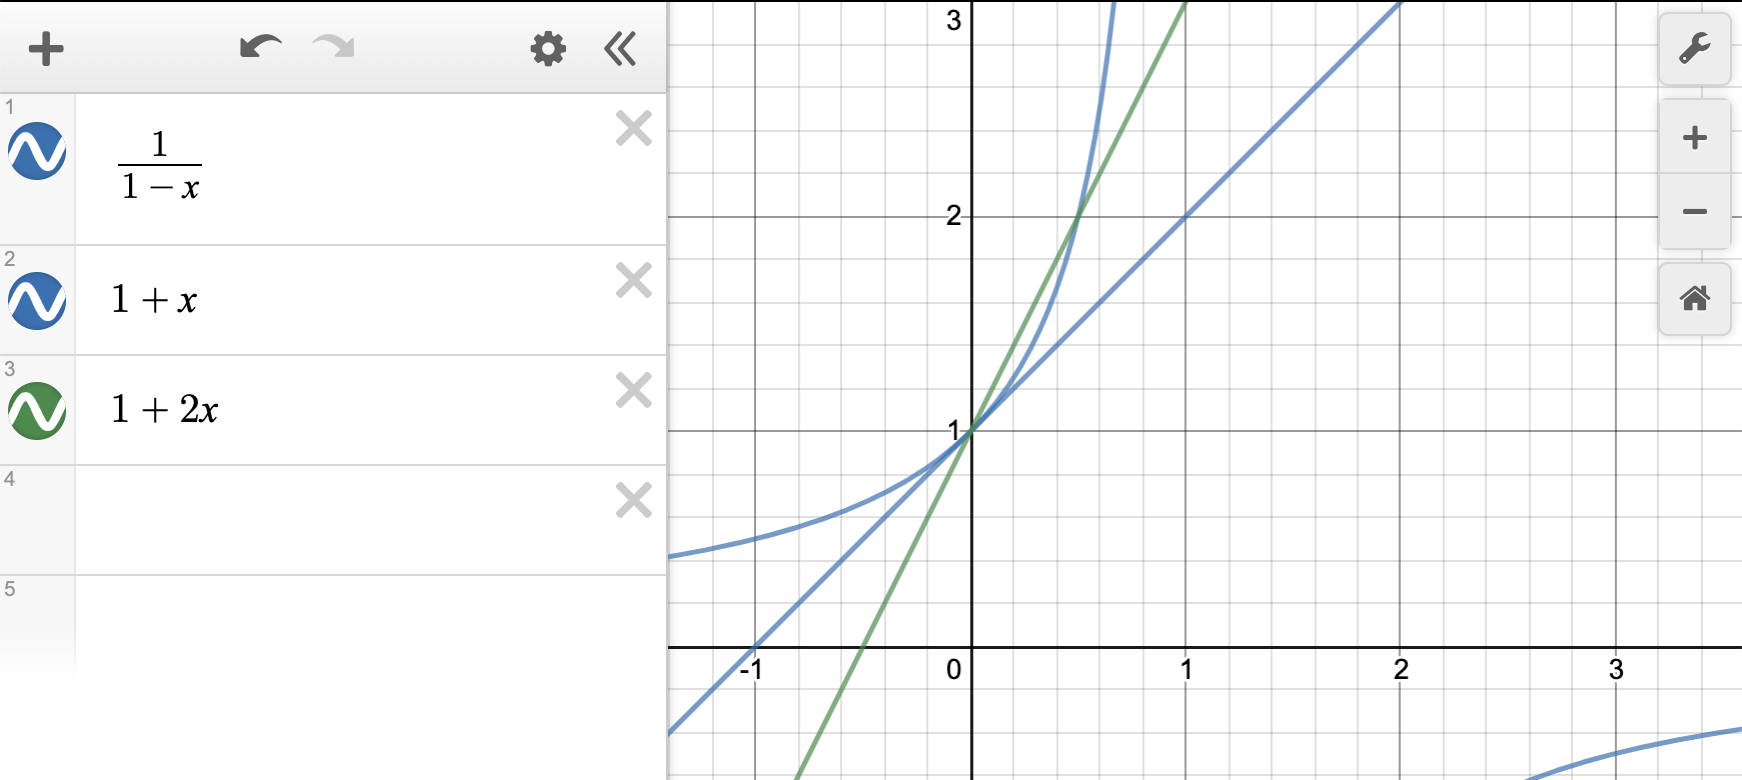
\includegraphics[width=\textwidth]{proof1.png}
\end{center}
\end{frame}

\begin{frame}
	\frametitle{example inequality}
	\begin{align*}
		1-\epsilon \leq \frac{1}{1+\epsilon} \leq 1 - .5\epsilon \text{ for } \epsilon \in [0,1].
	\end{align*}
	\textbf{Proof by plotting:}
	\begin{center}
		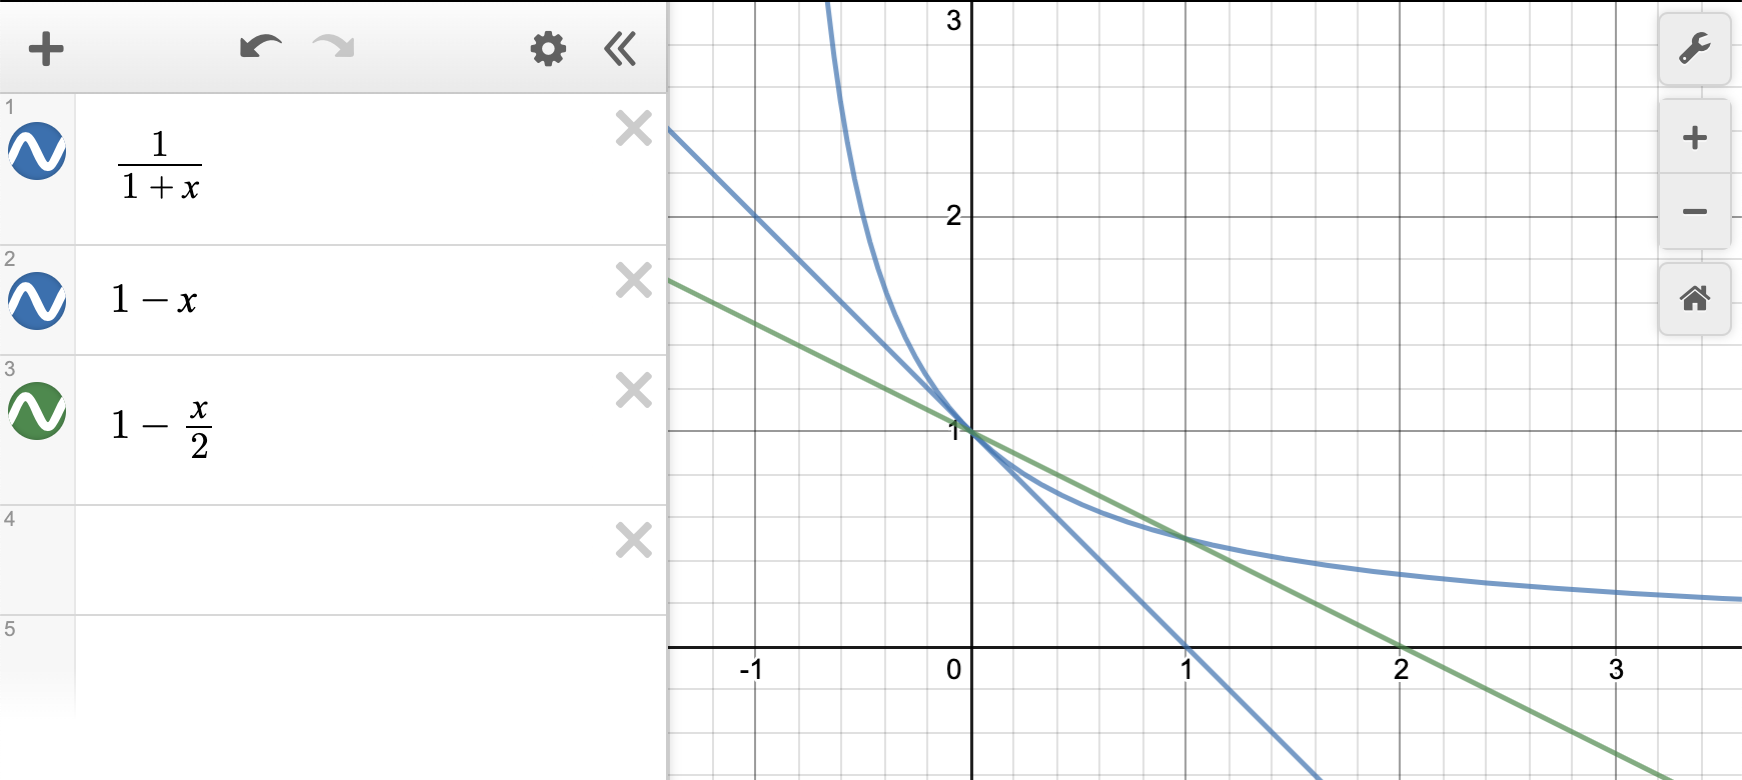
\includegraphics[width=\textwidth]{proof2.png}
	\end{center}
\end{frame}

\begin{frame} 
	\frametitle{general advice}
	\small
	\textbf{Tip:} When confronted with a complex expression, try to simplify by using big-Oh notation, or just rounding things off. Then clean-up your proof after you get to a solution.
	
	\textbf{Examples:}
	\begin{itemize}
		\item To start: $(m-1) \approx m$. \hspace{2.9em}Later: $m/2 \leq m-1 \leq m$. 
		\item To start: $\frac{1}{n} - \frac{1}{n^2} \approx \frac{1}{n}$. \hspace{3.5em}Later: $\frac{1}{2n} \leq \frac{1}{n} - \frac{1}{n^2} \leq \frac{1}{n}$.
		\item $\log(n/2)\approx \log(n)$
		\hspace{5em}Later: $\log(n)/2 \leq \log(n/2) \leq\log(n)$.
	\end{itemize}
\end{frame}

\begin{frame}
	\frametitle{definitions of variance}
	Suppose we have random variables $X_1, \ldots, X_k$. We say that $X_i$ and $X_j$ are \emph{independent} if, for all possible values $v_i, v_j$,
	\begin{align*}
			\Pr[X_i = v_i \text{ and } X_j = v_j] = 	\Pr[X_i = v_i]\cdot \Pr[X_j = v_j].
	\end{align*}
	We say $X_1, \ldots, X_k$ are \emph{pairwise independent} if $X_i,X_j$ are independent for all $i,j \in \{1, \ldots, k\}$.

\vspace{1em}
We say $X_1, \ldots, X_k$ are \emph{mutually independent} if, for all possible values $v_1, \ldots, v_k$,
		\begin{align*}
			\Pr[X_1 = v_1, \ldots, X_k = v_k] = 	\Pr[X_1 = v_1]\cdot\ldots \cdot\Pr[X_k = v_k].
		\end{align*}
	
	Mutual independence implies pairwise independence, but pairwise independence does not imply mutual independence. 
\end{frame}

\begin{frame}[t]
	\frametitle{definitions of variance}
		\begin{center}
		\textbf{\alert{Give an example of three random variables that are pairwise independent but not mutually independent.}}
	\end{center}
	 $X_1, \ldots, X_k$ are \emph{pairwise independent} if for all $i,j$, $v_i, v_j$, 
	 \begin{align*}
	 	\Pr[X_i = v_i \text{ and } X_j = v_j = 	\Pr[X_i = v_i]\cdot \Pr[X_j = v_j].
	 \end{align*}
 	$X_1, \ldots, X_k$ are \emph{mutually independent} if, for all $v_1, \ldots, v_k$,
	\begin{align*}
		\Pr[X_1 = v_1, \ldots, X_k = v_k] = 	\Pr[X_1 = v_1]\cdot\ldots \cdot\Pr[X_k = v_k].
	\end{align*}

\end{frame}



	\begin{frame}
	\frametitle{note on random hash functions}
	Let $h$ be a \emph{random function} from $|\mathcal{U}| \rightarrow \{1,\ldots, m\}$. This means that $h$ is constructed by an algorithm using a seed of random numbers, but then the function is fixed. Given input $x\in \mathcal{U}$, it always returns the same output, $h(x)$. 
	
	\textbf{Definition: Uniformly Random Hash Function.} 
	A random function $h: \mathcal{U}\rightarrow \{1, \ldots, m\}$ is called uniformly random if:
	\begin{itemize}
		\item $\Pr[h(x) = i] = \frac{1}{m}$ for all $x\in \mathcal{U}$, $i\in \{1,\ldots, m\}$.  
		\vspace{.5em}
		\item $h(x), h(y), h(z), \ldots$ are mutually independent random variables for all $x,y,z, \ldots \in \mathcal{U}$. 
		\begin{itemize}
			\vspace{.5em}
			\item Which implies that $\Pr[h(x) = h(y)] = $ 
		\end{itemize}
	\end{itemize}
	
	\vspace{2em}
	\begin{block}{\vspace*{-3ex}}
		\small $\mathcal{U} = $ universe of possible keys, $m=$ number of values hashed to.
	\end{block}
\end{frame}

	\begin{frame}[t]
	\frametitle{note on random hash functions}
	\begin{center}
	The only way to implement a \emph{truly} random hash function is to create a giant lookup table, where the numbers on the right are chosen independently at random from $\{1, \ldots, m\}$. 
	
		\begin{tabular}{c | c } 
		x & h(x) \\
		\hline 
		1 & 14\\ 
		2 & 25\\ 
		3 & 99\\ 
		4 & 16\\ 
		$\vdots$ & $\vdots$\\
		$|\mathcal{U}|$ & 87
		\end{tabular}
	\end{center}
If we're hashing 35 char ASCII strings (e.g. urls) the length of the table is \emph{greater than the number of atoms in the universe.}
	\end{frame}

	\begin{frame}[t]
	\frametitle{note on random hash functions}
	For the application to CountMin from last class we can weaken our assumption that $h$ is uniformly random.
	\begin{definition}[Universal hash function]
		A random hash function $h: \mathcal{U} \rightarrow \{1, \ldots, m\}$ is \emph{universal} if, for any fixed $x,y\in \mathcal{U}$,
		\begin{align*}
			\Pr[h(x) = h(y)] \leq \frac{1}{m}.
		\end{align*}
	\end{definition}
	\textbf{Claim:} A uniformly random hash-function is universal. 

\end{frame}

	\begin{frame}
	\frametitle{note on random hash functions}
	\begin{definition}[Universal hash function]
		A random hash function $h: \mathcal{U} \rightarrow \{1, \ldots, m\}$ is \emph{universal} if, for any fixed $x,y\in \mathcal{U}$,\vspace{-1.5em}
		\begin{align*}
			\Pr[h(x) = h(y)] \leq \frac{1}{m}.
		\end{align*}
	\end{definition}
	\textbf{Efficient alternative:} Let $p$ be a prime number between $|\mathcal{U}|$ and $2|\mathcal{U}|$. Let $a,b$ be random numbers in $0,\ldots, p$, $a\neq 0$.
	\begin{align*}
		h(x) = \left[a\cdot x + b \pmod{p}\right] \pmod{m}
	\end{align*} 
	is universal. Lecture notes with proof posted on website. 
	
	\begin{center}
	\textbf{How much space does this hash function take to store?}
	\end{center}
\end{frame}

\begin{frame}[t]
	\frametitle{note on random hash functions}
Similar alternative definition:
	\begin{definition}[Pairwise independent hash function]
		A random hash function $h: \mathcal{U} \rightarrow \{1, \ldots, m\}$ is pairwise independent if, for any fixed $x,y\in \mathcal{U}, i,j \in \{1\ldots, m\}$,
		\begin{align*}
			\Pr[h(x) = i \cap h(y) = j] = \frac{1}{m^2}.
		\end{align*}
	\end{definition}
\vspace{-1em}
Basically same construction as universal hash, except we don't restrict $a \neq 0$ and need to be careful about rounding.

	Can naturally be extended to $k$-wise independence for $k > 2$, which is strictly stronger, and needed for some applications. 
	\begin{align*}
		\Pr[h(u_1) = v_1 \cap h(u_2) = v_2 \cap \ldots h(u_k) = v_k] = \frac{1}{m^k}, 
	\end{align*}
for all $u_1, \ldots, u_k \in \mathcal{U}$ and $v_1, \ldots, v_k \in \{1, \ldots, m\}$.
\end{frame}

\begin{frame}
	\frametitle{lecture road map}
	Last week we saw the power of \emph{Linearity of Expectation} + \emph{Markov's}. This week we will discuss four more tools:
	\begin{itemize}
		\item \emph{Linearity of Variance} + \emph{Chebyshev's Inequality}
		\item \emph{Union Bound} + \emph{Exponential Tail Bounds}
	\end{itemize}
	\begin{center}
		
\includegraphics[width=.5\textwidth]{4function.png}
		
		\textbf{\alert{These six simple tools combined are surprising powerful and flexible. They form the cornerstone of randomized algorithm design.}}
	\end{center}
 \end{frame}

\begin{frame}
	\frametitle{chebyshev's inequality}
	\small
	A new concentration inequality:
	\begin{lemma}[Chebyshev's Inequality]
		Let $X$ be a random variable with expectation $\E[X]$ and variance $\sigma^2 = \Var[X]$. Then for any $k > 0$,
		\begin{align*}
			\Pr[|X - \E[X]| \geq k\cdot\sigma] \leq \frac{1}{k^2}
		\end{align*}
	\end{lemma}
	\vspace{-.5em}
	\begin{center}
		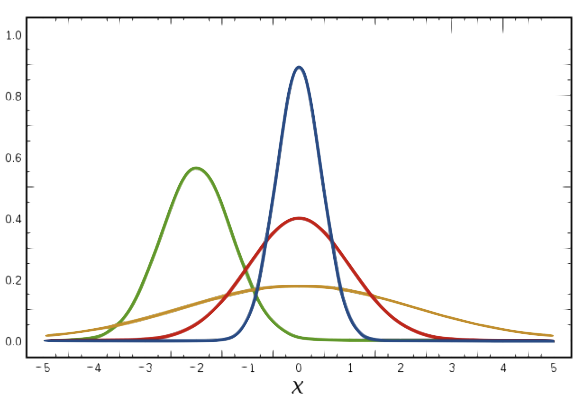
\includegraphics[width=.4\textwidth]{rvs.png}
		
		$\sigma = \sqrt{\Var[X]}$ is the \emph{standard deviation} of $X$. Intuitively this bound makes sense: it is {tighter} when $\sigma$ is smaller.
	\end{center}
	%\vspace{-2em}
	%	\begin{block}{\vspace*{-3ex}}
	%		\small
	%		Recall, $\Var[X] = \E[(X - \E[X])^2] = \E[X^2] - \E[X]^2$.
	%	\end{block}
\end{frame}

\begin{frame}
	\frametitle{comparison to markov's inequality}
	\small
	Properties of Chebyshev's inequality:
	\begin{itemize}
		\item \textbf{Good:} No requirement of non-negativity. $X$ can be anything.
		\item \textbf{Good:} Two-sided. Bounds the probability that $|X - \E X|$ is large, which means that $X$ isn't too far above \emph{or} below its expectation. Markov's only bounded probability that $X$ exceeds $\E[X]$.
		\item \textbf{Bad/Good:} Requires a bound on the variance of of $X$.  
	\end{itemize}
	\alert{\textbf{No hard rule for which to apply! Both Markov's and Chebyshev's are useful in different settings.}}
\end{frame} 

\begin{frame}
	\frametitle{proof of chebyshev's inequality}
	\small
	\textbf{Idea:} Apply Markov's inequality to the (non-negative) random variable $S = (X-\E[X])^2$.
	\begin{lemma}[Chebyshev's Inequality]
		Let $X$ be a random variable with expectation $\E[X]$ and variance $\sigma^2 = \Var[X]$. Then for any $k > 0$,
		\begin{align*}
			\Pr[|X - \E[X]| \geq k\cdot\sigma] \leq \frac{1}{k^2}
		\end{align*}
	\end{lemma}
%	\begin{align*}
%		\Pr[S \geq k^2\sigma^2] &\leq \frac{\E[S]}{k^2\sigma^2} \text{\hspace{2em}\blue{(Markov inequality)}}\\
%		\Pr[\sqrt{S} \geq k\sigma] &\leq \frac{\E[(X-\E[X])^2]}{k^2\sigma^2}\\
%		\Pr[|X - \E[X]|\geq k\sigma] &\leq \frac{\sigma^2}{k^2\sigma^2} = \frac{1}{k^2}.\qed
%	\end{align*}
	
	\vspace{7em}
	\begin{block}{\vspace*{-3ex}}
		\small \textbf{Markov's inequality}: for non-negative r.v. $S$, $\Pr[S \geq t] \leq \E[S]/t$.  
	\end{block}
\end{frame}

\begin{frame}
	\frametitle{quick example}
	\begin{center}
	\textbf{If I flip a fair coin $100$ times, show that with $93\%$ chance I get between $30$ and $70$ heads?}
	\end{center}
	Let $C_1, \ldots, C_{100}$ be independent random variables that are $1$ with probability $1/2$, $0$ otherwise.

	Let $H = \sum_{i=1}^{100} C_i$ be the number of heads that get flipped.	
	
	\begin{align*}
		\E[H] = \hspace{20em}
	\end{align*}

	\begin{align*}
	\Var[H] = \hspace{20em}
	\end{align*}
\vspace{4em}
\end{frame}

\begin{frame}
	\frametitle{linearity of variance}
	\textbf{Fact:} For \emph{pairwise independent}\footnote{Technically, pairwise uncorrelated suffices, which is a slightly weaker assumption.} random variables $X_1, \ldots, X_m$, 
	\begin{align*}
		\Var[X_1 + X_2 + \ldots + X_m] = 	\Var[X_1]+ \Var[X_2] + \ldots + \Var[X_m]. 
	\end{align*}
I.e., we require that for any $i,j$ $X_i$ and $X_j$ are independent. 

This is strictly weaker than \emph{mutual independence}, which requires that for all possible values $v_1, \ldots, v_k$,
\begin{align*}
	\Pr[X_1 = v_1, \ldots, X_k = v_k] = 	\Pr[X_1 = v_1]\cdot\ldots \cdot\Pr[X_k = v_k].
\end{align*}
\end{frame}

\begin{frame}
	\frametitle{quick example}
	\begin{center}
		\textbf{If I flip a fair coin $100$ times, show that with $93\%$ chance I get between $30$ and $70$ heads?}
	\end{center}
	Let $C_1, \ldots, C_{100}$ be independent random variables that are $1$ with probability $1/2$, $0$ otherwise.
	
	Let $H = \sum_{i=1}^{100} C_i$ be the number of heads that get flipped.	
	
	$\Var[H] = 25$.  
	
	\textbf{Chebyshev's:}

	\vspace{4em}
\end{frame}

%\begin{frame}
%	\frametitle{out of class exercise}
%	Recall the set up from last lecture:
%	
%	Draw items $x_1, \ldots, x_m$ uniformly at random from a set of size $n$ and count the number of collisions:
%	\begin{align*}
%		D &= \sum_{\substack{i,j \in \{1,\ldots, m\}\\ i < j}} \mathbbm{1}[x_i == x_j]. 
%	\end{align*}
%	
%	We showed that $\E[D] = {m \choose 2}\frac{1}{n}$. 
%	
%	\textbf{Exercise:} Show that $\Var[D] \leq {m \choose 2}\frac{1}{n}$ and use to prove the claim on Slide 32 from Lecture 1. 
%	
%\end{frame}


\begin{frame}
	\frametitle{streaming algorithms}
	\textbf{Abstract architecture of a streaming algorithm:} 
	
	Have massive dataset $X = {x_1, \ldots, x_n}$ with $n$ pieces of data that arrive in a sequential stream. There is far too much data to store or process it in a single location.
	\begin{itemize}
		\item Still want to analyze the data: i.e. fit a model or (approximately) compute some function $f(X)$.
		\item To do so, we must compress data ``on-the-fly'', storing some smaller data structure which still contains interesting information.
		\item Often can only take a \emph{single-pass} over the data. 
	\end{itemize}
\begin{center}
	\textbf{Count-Min} was our first example of a streaming algorithm for the $(\epsilon,k)$-frequent items problem. 
\end{center}
\end{frame}

\begin{frame}
	\frametitle{streaming algorithms in practice}
	\textbf{Sensor data:} GPS or seismometer readings to detect geological anomalies, telescope images, satellite imagery, highway travel time sensors.
	
	\textbf{Web traffic and data:} User data for website, including e.g. click data, web searches and API queries, posts and image uploads on social media.
	
	\textbf{Training machine learning models:} Often done in a streaming setting when training dataset is huge, often with multiple passes.
	\begin{center}
		
\includegraphics[width=.8\textwidth]{streamFrameworks.png}
		
		Lots of software frameworks exist for easy development of streaming algorithms.
	\end{center}
\end{frame}

\begin{frame}
	\frametitle{distinct elements problem}
	\textbf{Input:} $x_1, \ldots, x_n \in \mathcal{U}$ where $\mathcal{U}$ is a huge universe of items. 
	
	\textbf{Output:} Number of \emph{distinct} inputs.
	
	\textbf{Example:} $f(1, 10, 2, 4, 9, 2, 10, 4) \rightarrow 5$
	
	\vspace{.5em}
	\hrule
	\vspace{.5em}
	
		\textbf{Applications}:
			\begin{itemize}
				\item Distinct users hitting a webpage. 
				\item Distinct values in a database column (e.g. for estimating the size of group by queries)
				\item Number of distinct queries to a search engine.
				\item Distinct motifs in DNA sequence.
			\end{itemize}
		Implementations widely used at Google (Sawzall, Dremel, PowerDrill), Twitter, Facebook (Presto), etc. 
\end{frame}

\begin{frame}[t]
	\frametitle{distinct elements problem}
	\textbf{Input:} $d_1, \ldots, d_n \in \mathcal{U}$ where $\mathcal{U}$ is a huge universe of items. 
	
	\textbf{Output:} Number of \emph{distinct} inputs, $D$.
	
	\textbf{Example:} $f(1, 10, 2, 4, 9, 2, 10, 4) \rightarrow D = 5$
	
	\vspace{.5em}
	\hrule
	\vspace{.5em}
	
	\textbf{Naive Approach}:
	Store a dictionary of all items seen so far. Takes $O(D)$ space. We will aim to do a lot better than that. 
	
	\vspace{1em}
	\textbf{Goal:} Return $\tilde{D}$ satisfying $(1-\epsilon) D \leq \tilde{D} \leq (1+\epsilon) D$ and only used $O(1/\epsilon^2)$ space.

\end{frame}

\begin{frame}
	\frametitle{distinct elements problem}
\textbf{Input:} $d_1, \ldots, d_n \in \mathcal{U}$ where $\mathcal{U}$ is a huge universe of items. 

	\textbf{Output:} Number of \emph{distinct} inputs, $D$.

\textbf{Example:} $f(1, 10, 2, 4, 9, 2, 10, 4) \rightarrow D = 5$

\vspace{.5em}
\hrule
\vspace{.5em}

\textbf{Flajolet–Martin (simplified)}:
\begin{itemize}
	\item Choose random hash function $h: \mathcal{U} \rightarrow [0,1]$.
	\item $S = 1$ 
	\item For $i = 1, \ldots, n$
	\begin{itemize}
		\item $S \leftarrow \min(S, h(x_i))$
	\end{itemize} 
	\item Return: $\frac{1}{S} - 1$
\end{itemize}
\end{frame}

\begin{frame}
	\frametitle{hold up...}
	\begin{center}
	The hash function $h$ maps from $\mathcal{U}$ to a random point in $[0,1]$?
	\end{center}

	\textbf{Hashing to real numbers:}
	\begin{itemize}
		\item Impossible to implement $h(x)$ in reality, but you can replace it with $\frac{g(x)}{k}$, where $g$ is a hash function that maps to $\{0,1,\ldots,k\}$ for sufficiently large $k$.
		\item All results hold if this ``discrete'' hash is used instead, but the analysis is simpler if we assume access to $h$.
		\item Just like when we assumed uniform random hash functions, this is a useful abstraction which makes understanding and analyzing algorithms easier. 
	\end{itemize}
\end{frame}

\begin{frame}
	\frametitle{visualization}
	\small
	\textbf{Flajolet–Martin (simplified)}:
	\vspace{-.5em}
	\begin{itemize}
		\item Choose random hash function $h: \mathcal{U} \rightarrow [0,1]$.
		\vspace{-.25em}
		\item $S = 1$ 
		\vspace{-.25em}
		\item For $i = 1, \ldots, n$
		\vspace{-.25em}
		\begin{itemize}
			\vspace{-.25em}
			\item $S \leftarrow \min(S, h(x_i))$
		\end{itemize} 
		\vspace{-.25em}
		\item Return: $\tilde{D} = \frac{1}{S} - 1$
	\end{itemize}
\vspace{-.5em}
	\begin{center}
	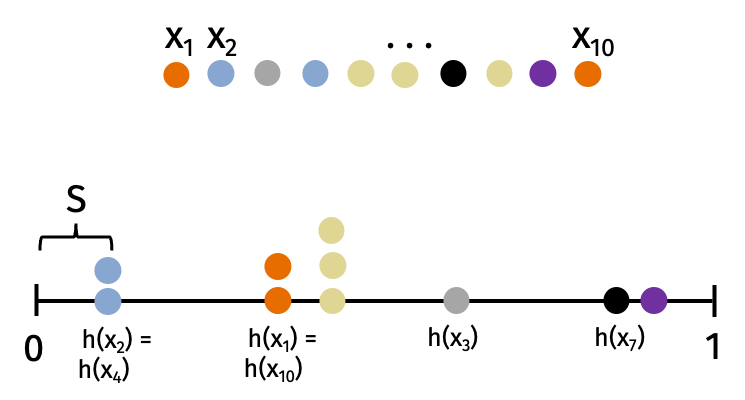
\includegraphics[width=.75\textwidth]{better_minhash_cut.png}
	\end{center}
\end{frame}


\begin{frame}
	\frametitle{fm analysis}	
	Let $D$ equal the number of distinct elements in our stream.
	\begin{center}
	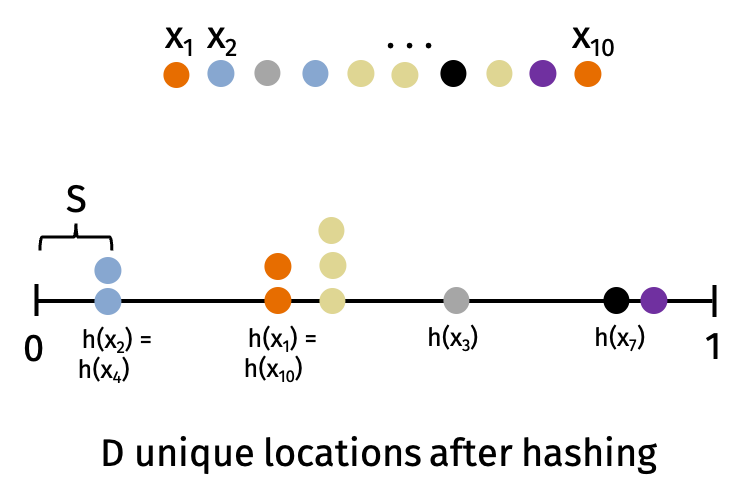
\includegraphics[width=.7\textwidth]{better_minhash.png}
	\end{center}
	\textbf{Intuition:} When $D$ is larger, $S$ will be smaller. Makes sense to return the estimate $\tilde{D} = \frac{1}{S}-1$.
\end{frame}

\begin{frame}
	\frametitle{fm analysis}	
	\textbf{What is $\E S$?}
	\begin{center}
		\uncover<2->{
			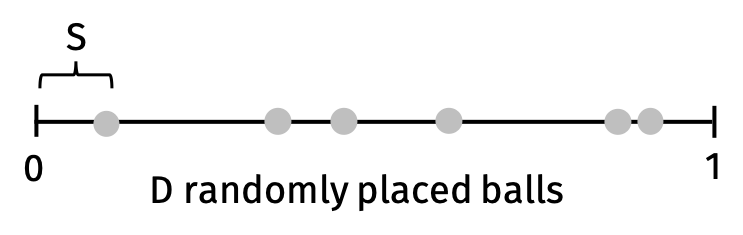
\includegraphics[width=.6\textwidth]{FMimage.png}
		}
	\end{center}
	
	\uncover<3->{
		Let $D$ equal the number of distinct elements in our stream.
		\begin{lemma}
			$\E S = \frac{1}{D + 1}$.
		\end{lemma}
		\vspace{3em}
	}
\end{frame}

\begin{frame}
	\frametitle{the calculus proof}
	\textbf{Proof:} 
	\begin{align*}
		\E[S] &= \int_0^1 \Pr[S \geq \lambda] d\lambda & &\text{Exercise: Why?} \\
		&= \int_0^1 (1-\lambda)^D d\lambda & &\text{} \\
		& = \frac{-(1-\lambda)^{D+1}}{D+1}\Bigm|_{\lambda=0}^1\\
		& = \frac{1}{D+1}
	\end{align*}
\end{frame}



\begin{frame}
	\frametitle{proof ``from the book''}
	$\E[S] = \Pr[(D+1)^\text{st} \text{ item has the smallest hash value}]$.
	\begin{center}
		\uncover<2->{
			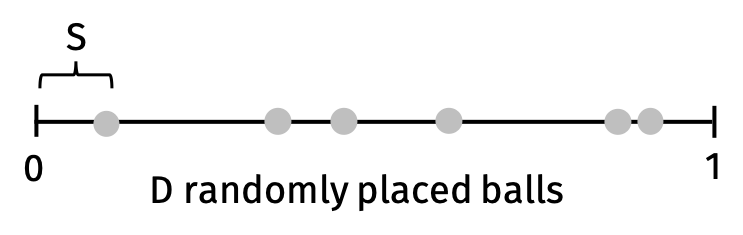
\includegraphics[width=.6\textwidth]{FMimage.png}
		}
	\end{center}
\textbf{Formally, we are using the fact that:}
	\begin{align*}
		&\Pr[A] = \E_{h_1, \ldots, h_D}\left[\Pr\left[A\mid h_1, \ldots, h_D\right]\right]
	\end{align*}
	
\end{frame}

\begin{frame}
	\frametitle{proof ``from the book''}
	$\E[S] = \Pr[(D+1)^\text{st} \text{ item has the smallest hash value}]$.
	\begin{center}
		\uncover<2->{
			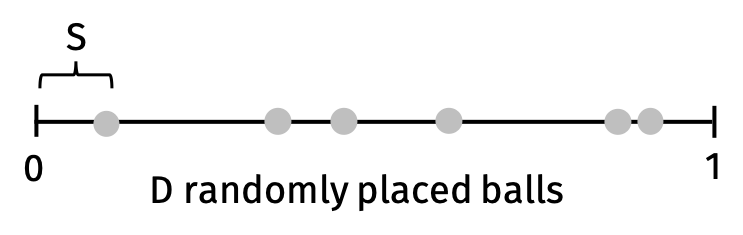
\includegraphics[width=.6\textwidth]{FMimage.png}
		}
	\end{center}
	By symmetry, this equals $\frac{1}{D+1}$ (since every ball is equally likely to be first). 
	
\end{frame}


\begin{frame}
	\frametitle{proving concentration}	
	$\E S = \frac{1}{D + 1}$. \textbf{Estimate:} $\tilde{D} = \frac{1}{S} - 1$. We have for $\epsilon < \frac{1}{2}$:
	
	\begin{center}
	If $(1-\epsilon)\E S \leq S \leq (1+\epsilon)\E S$, then:
	\begin{align*}
	\alert{(1-4\epsilon)D \leq \tilde{D} \leq (1+4\epsilon)D.}
	\end{align*}
	\end{center}
\vspace{10em}

	So, it suffices to show that $S$ concentrates around its mean. I.e. that $|S - \E S| \leq \epsilon\cdot\E S$. We will use Chebyshev's inequality as our concentration bound.
\end{frame}

\begin{frame}
	\frametitle{calculus proof}	
	\begin{lemma}
	$\Var[S] = \E [S^2] - \E[S]^2= \frac{2}{(D+1)(D+2)} - \frac{1}{(D+1)^2} \leq \frac{1}{(D+1)^2}$.
	\end{lemma}
	\textbf{Proof:} 
	\begin{align*}
	\E[S^2] &= \int_0^1 \Pr[S^2 \geq \lambda] d\lambda & &\text{} \\
	&= \int_0^1 \Pr[S \geq \sqrt{\lambda}] d\lambda & &\text{} \\
	&= \int_0^1 (1-\sqrt{\lambda})^D d\lambda & &\text{} \\
	& = \frac{2}{(D+1)(D+2)}& &\text{}
	\end{align*}
	
	\small
	\url{www.wolframalpha.com/input/?i=integral+from+0+to+1+of+\%281-sqrt\%28x\%29\%29\%5ED}
\end{frame}

\begin{frame}
	\frametitle{proof ``from the book''}
	$\E[S^2] = ??$.
	\begin{center}
		\uncover<2->{
			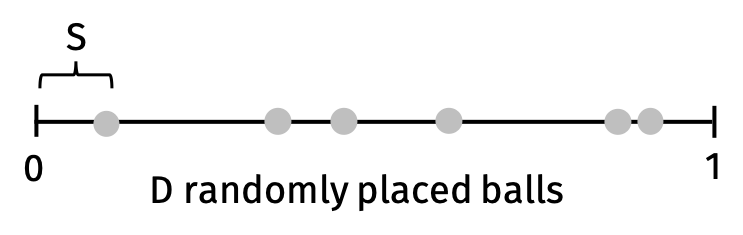
\includegraphics[width=.6\textwidth]{FMimage.png}
		}
	\end{center}
\end{frame}

\begin{frame}
	\frametitle{fm analysis}
	\begin{itemize}
		\item $\E[S] = \frac{1}{D+1} = \mu.$
		\item $\Var[S] \leq \frac{1}{(D+1)^2} = \mu^2$. Standard deviation: $\sigma \leq \mu$.
		\item Want to bound $\Pr[|S - \mu| \geq \epsilon \mu] \leq \delta$.
	\end{itemize}
	
	\textbf{Chebyshev's}: $\Pr[|S - \mu| \geq \epsilon \mu] = \Pr[|S - \mu| \geq \epsilon \sigma] \leq \frac{1}{\epsilon^2}$.
	
	\begin{center}
	\alert{\textbf{Vacuous bound. Our variance is way too high!}}
	\end{center}
\end{frame}


\begin{frame}
	\frametitle{variance reduction}
	\textbf{Trick of the trade:} Repeat many independent trials and take the mean to get a better estimator.
	
	Given i.i.d. (independent, identically distributed) random variables $X_1, \ldots, X_k$ with mean $\mu$ and variance $\sigma^2$, what is:
	\begin{itemize}
		\item $\E\left[\frac{1}{k}\sum_{i=1}^k X_i\right] = $
		\vspace{1em}
		\item $\Var\left[\frac{1}{k}\sum_{i=1}^k X_i\right] = $
	\end{itemize} 
\end{frame}

\begin{frame}
	\frametitle{fm analysis}
	Using independent hash functions, maintain $k$ independent sketches $S_1, \ldots, S_k$.
\vspace{-1em}
\begin{center}
	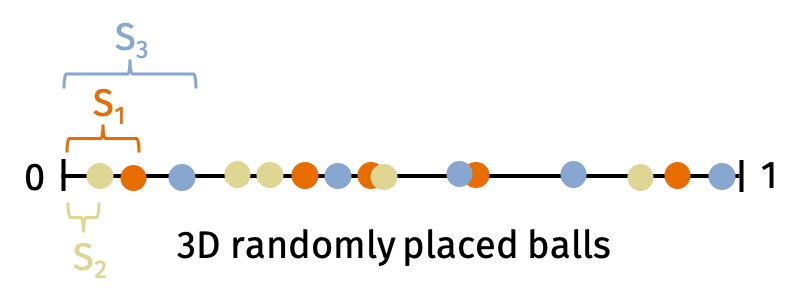
\includegraphics[width=.7\textwidth]{improvedFM.png}
\end{center}

\vspace{-1em}	
\textbf{Flajolet–Martin}:
		\begin{itemize}
			\item Choose $k$ random hash function $h_1, \ldots, h_k: \mathcal{U} \rightarrow [0,1]$.
			\item $S_1 = 1, \ldots, S_k = 1$ 
			\item For $i = 1, \ldots, n$
			\begin{itemize}
				\item $S_j \leftarrow \min(S_j, h_j(x_i))$ for all $j \in 1, \ldots, k$.
			\end{itemize} 
			\item $S = (S_1 + \ldots + S_k)/k$
			\item Return: $\frac{1}{S} - 1$
		\end{itemize}
\end{frame}

\begin{frame}
	\frametitle{fm analysis}
	\textbf{1 estimator}:
	\begin{itemize}
		\item $\E[S] = \frac{1}{D+1} = \mu.$
		\item $\Var[S] = \mu^2$
	\end{itemize}
	\textbf{$k$ estimators}:
	\begin{itemize}
		\item $\E[S] = \frac{1}{D+1} = \mu.$
		\item $\Var[S] \leq  \mu^2/k$
		\item By Chebyshev, $\Pr[|S - \E S| \geq c \mu/\sqrt{k}] \leq \frac{1}{c^2}$.
	\end{itemize}

	Setting $c = 1/\sqrt{\delta}$ and $k = \frac{1}{\epsilon^2\delta}$ gives:
	\begin{align*}
		\Pr[|S - \mu| \geq \epsilon \mu] \leq \delta.
	\end{align*}


\textbf{Total space complexity}: $\alert{O\left(\frac{1}{\epsilon^2\delta}\right)}$ to estimate distinct elements up to error $\epsilon$ with success probability $1-\delta$.
\end{frame}

\begin{frame}[t]
	\frametitle{fm analysis}
	\textbf{Total space complexity}: $\alert{O\left(\frac{1}{\epsilon^2\delta}\right)}$ to estimate distinct elements up to error $\epsilon$ with success probability $1-\delta$.
	
	\begin{itemize}
		\item Recall that to ensure $(1-\bar{\epsilon}) D \leq \frac{1}{S} - 1 \leq (1+\bar{\epsilon}) D$, we needed  $|S - \mu| \leq \frac{\bar{\epsilon}}{4} \mu$. 
		\item So apply the result from the previous slide with $\epsilon = \bar{\epsilon}/4$. 
		\item Need to store $k = \frac{1}{\epsilon^2\delta} = \frac{1}{(\bar{\epsilon}/4)^2\delta} = \frac{16}{\epsilon^2\delta}$ counters.
	\end{itemize}
\end{frame}

\begin{frame}
	\frametitle{note on failure probability}
	$\alert{O\left(\frac{1}{\epsilon^2\delta}\right)}$ space is an impressive bound:
	\begin{itemize}
		\item $1/\epsilon^2$ dependence cannot be improved.
		\item No linear dependence on number of distinct elements $D$.\footnote{Technically, we need to store the hash functions $h_1, \ldots, h_k$, which each take $O(\log |\mathcal{U}|) \geq O(\log |\mathcal{D}|)$ space. So if we are more careful, the space complexity is $O\left(\frac{\log D}{\epsilon^2\delta}\right)$.}
		\item But... $1/\delta$ dependence is not ideal. For $95\%$ success rate, pay a $\frac{1}{5\%} = 20$ factor overhead in space. 
	\end{itemize}
We can get a better bound depending on $O(\log(1/\delta))$ using \emph{exponential tail bounds.}
\end{frame}

\begin{frame}
	\frametitle{distinct elements in practice}
	In practice, we cannot hash to real numbers on $[0,1]$. Instead, map to bit vectors.
	
	\textbf{Real Flajolet-Martin / HyperLogLog:}
	\begin{columns}
		\begin{column}{.4\textwidth}
			\begin{center}
				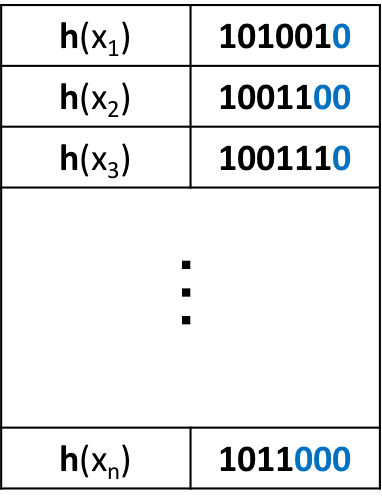
\includegraphics[width=.7\textwidth]{loglog2.png}
			\end{center}
		\end{column}
		\begin{column}{.6\textwidth}
				\begin{itemize}
					\item Estimate \# distinct elements based on maximum number of trailing zeros $\bv m$.
					\item The more distinct hashes we see, the higher we expect this maximum to be.
				\end{itemize}
		\end{column}
	\end{columns}
	\begin{center}
	\end{center}
\end{frame}

\begin{frame}
	\frametitle{loglog space}
	\textbf{Total Space:} $O \left (\frac{\log \log D}{\epsilon^2} + \log D \right )$ for an $\epsilon$ approximate count.
	
	\small ``Using an auxiliary memory smaller than the size of this abstract, the LogLog algorithm makes it possible to estimate in a single pass and within a few percents the number of different words in the whole of Shakespeare’s works.'' -- Flajolet, Durand.
	
	
	\vspace{1em}
	\uncover<3->{
		Using HyperLogLog to count $1$ billion distinct items with $2\%$ accuracy:
		\begin{align*}
			\text{space used } &= O \left (\frac{\log \log D}{\epsilon^2} + \log D \right )\\ \uncover<2->{&= \frac{1.04 \cdot \lceil \log_2 \log_2 D\rceil}{\epsilon^2} + \lceil \log_2 D \rceil \text{ bits}\\}
			\uncover<3->{&= \frac{1.04 \cdot 5}{.02^2} + 30 = 13030\text{ bits} \approx \alert{1.6\ kB}!}
		\end{align*}
	}
\end{frame}

\begin{frame}
	\frametitle{hyperloglog in practice}
	\begin{center} 
		Although, to be fair, storing a dictionary with $1$ billion bits only takes 125 megabytes. No tiny, but not unreasonable.
		
		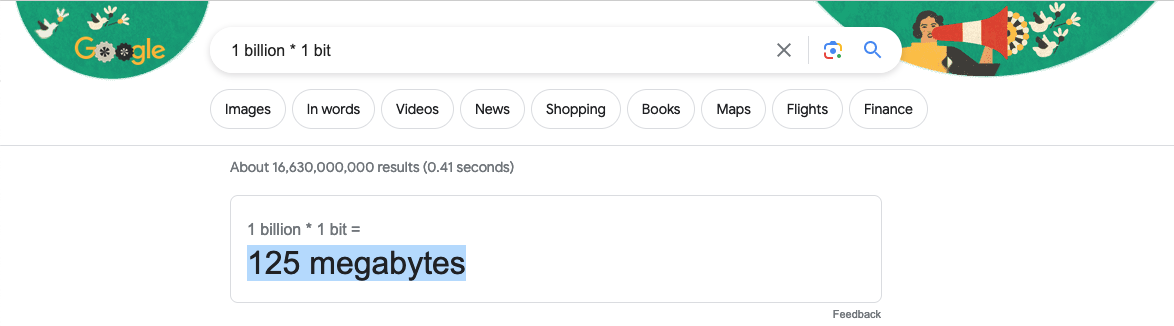
\includegraphics[width=\textwidth]{google_bit_calculations.png}
	\end{center}
	The real value in distinct elements sketches is in more complex applications than a simple stream.
\end{frame}

\begin{frame}
	\frametitle{distributed distinct elements}
	\begin{center}
		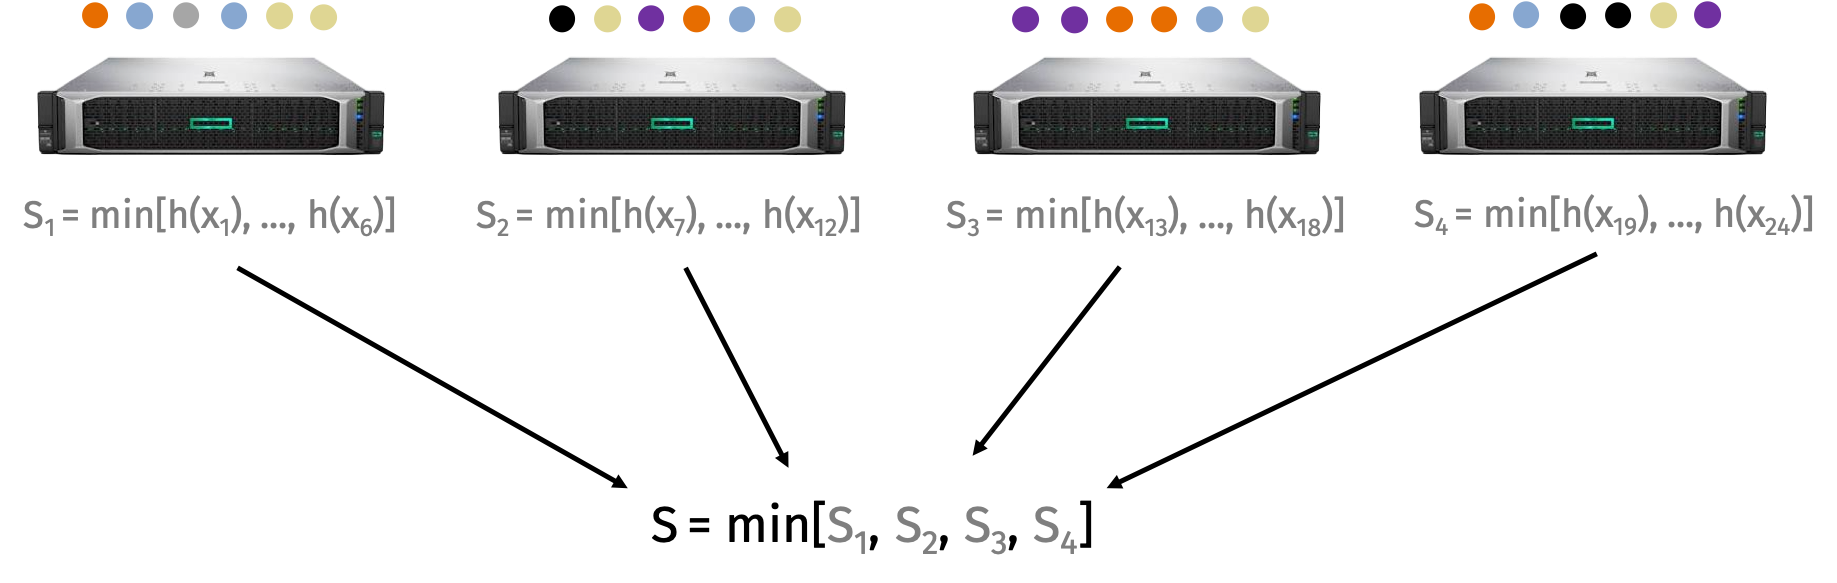
\includegraphics[width=\textwidth]{dist_min_hash.png}
	\end{center}

	Distinct elements summaries are ``mergeable''. No need to share lists of distinct elements if those elements are stored on different machines. Just share minimum hash value.
\end{frame}

\begin{frame}
	\frametitle{hyperloglog in practice}
	\small
	\textbf{Implementations:} Google PowerDrill, Facebook Presto, Twitter Algebird, Amazon Redshift.
	
	\textbf{Use Case:} Exploratory SQL-like queries on tables with $100$'s of billions of rows.
	\begin{itemize}
		\item \alert{Count} number of \alert{distinct} users in Germany that  made at least one search containing the word `auto' in the last month.
		\item \alert{Count} number of \alert{distinct} subject lines in emails sent by users that have registered in the last week, in comparison to number of emails sent overall (to estimate rates of spam accounts).
		% \item \alert{Count} number of \alert{distinct} zip codes in which at least one search has been made for blah
	\end{itemize}
	\uncover<2->{
		\begin{center}
			\textbf{Answering a query requires a (distributed) linear scan over the database: \emph{2 seconds} in Google's distributed implementation.}
			
				\textbf{\alert{Google Paper: ``Processing a Trillion Cells per Mouse Click''}}
		\end{center}
	}
\end{frame}

%\begin{frame}
%	\frametitle{hyperloglog in practice}
%	\textbf{Google Paper: ``Processing a Trillion Cells per Mouse Click''}
%	
%	``The system has been in production since end of 2008 and
%	was made available for internal users across all of Google
%	mid 2009. Each month it is used by more than 800 users
%	sending out about 4 million SQL queries. \textbf{\alert{After a hard day’s
%			work, one of our top users has spent over 6 hours in the
%			UI, triggering up to 12 thousand queries.}} When using our
%	column-store as a backend, this may amount to scanning as
%	much as 525 trillion cells in (hypothetical) full scans.''
%\end{frame}

\begin{frame}[standout]
	\begin{center}
		break
	\end{center}
\end{frame}


\begin{frame}
	\frametitle{load balancing}
	\textbf{Load balancing problem:}
	
	Suppose Google answers map search queries using servers $A_1, \ldots, A_q$. Given a query like ``new york to rhode island'', common practice is to choose a random hash function $h \rightarrow \{1\ldots, q\}$ and to route this query to server:
	\begin{align*}
		A_{h(\text{``new york to rhode island'})}
	\end{align*}

	\textbf{Goal:} Ensure that requests are distributed evenly, so no one server gets loaded with too many requests. We want to avoid  downtime and slow responses to clients. 
	
	\begin{center}
		\alert{\textbf{Why use a hash function instead of just distributing requests randomly?}}
	\end{center}
	

\end{frame}

\begin{frame}
	\frametitle{load balancing}
	Suppose we have $n$ servers and $m$ requests, $x_1,\ldots, x_m$. Let $s_i$ be the number of requests sent to server $i \in \{1,\ldots, n\}$ :
	\begin{align*}
		s_i = \sum_{j=1}^m \mathbbm{1}[h(x_j) = i]. 
	\end{align*}
	
	Formally, our goal is to understand the value of maximum load on any server, which can be written as the random variable:
	\begin{align*}
		S = \max_{i\in \{1,\ldots, n\}} s_i.
	\end{align*}	
\end{frame}

\begin{frame}
	\frametitle{load balancing}
	A good first step in any analysis of random variables is to first think about expectations. 
	If we have $n$ servers and $m$ requests, for any $i\in \{1,\ldots, n\}$:
	\begin{align*}
		\E[s_i] = \sum_{j=1}^m \E\left[\mathbbm{1}[h(x_j) = i]\right] = \frac{m}{n}.
	\end{align*}
	
	But it's very unclear what the expectation of $S = \max_{i\in \{1,\ldots, n\}} s_i$ is... in particular, $\E[S] \alert{\neq} \max_{i\in \{1,\ldots, n\}} \E[s_i]$. 
	
	\textbf{Exercise:} Convince yourself that for two random variables $A$ and $B$, $\E[\max(A,B)] \neq \max(\E[A], \E[B])$ even if those random variable are independent. 
\end{frame}

\begin{frame}
	\frametitle{simplifying assumptions}
	\textbf{Number of servers:} To reduce notation and keep the math simple, let's assume that $m = n$. I.e., we have exactly the same number of servers and requests. 
	
	\textbf{Hash function:} Continue to assume a fully (uniformly) random hash function $h$.
	
	\begin{center}
		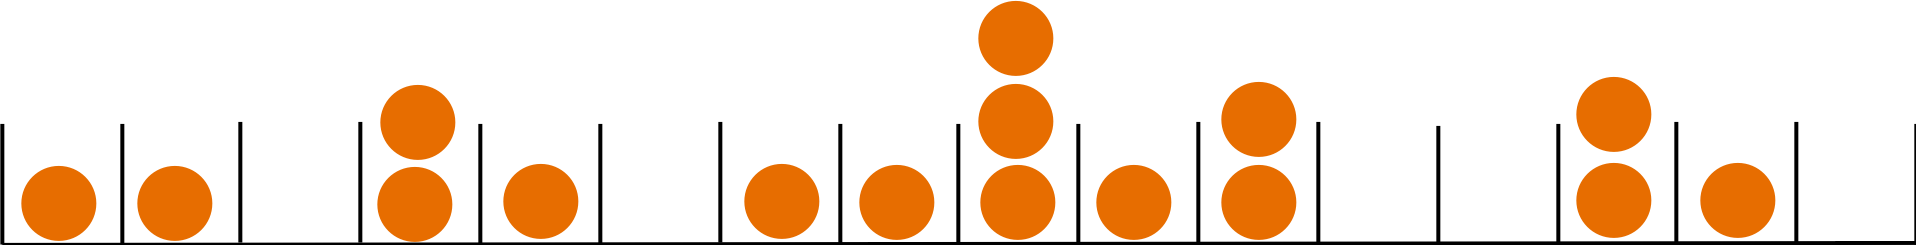
\includegraphics[width=.8\textwidth]{balls_into_bins.png}
		
		Often called the ``balls-into-bins'' model. 
	\end{center}
	
	$\E[s_i] = $ expected number of balls per bin $=\frac{m}{n} = 1$. We would like to prove a bound of the form:
	\begin{align*}
		\Pr[\max_i s_i \geq C] \leq \frac{1}{10}. 
	\end{align*}
	for as tight a value of $C$. I.e., something much better than $C = n$. 
\end{frame}

\begin{frame}
	\frametitle{bounding a union of events}
	\textbf{Goal:} Prove that for some $C$,
	\begin{align*}
		\Pr[\max_i s_i \geq C] \leq \frac{1}{10}. 
	\end{align*}
	 $\cap$ means ``and''. $\cup$ means ``or''.
	
	\textbf{Equivalent statement:} Prove that for some $C$, 
	\begin{align*}
		\Pr[(s_1 \geq C) \cup (s_2 \geq C) \cup \ldots \cup (s_n \geq C)] \leq \frac{1}{10}. 
	\end{align*}
	
	\begin{center}
		\textbf{\alert{Need to bound the probability of a \emph{union} of different events.}}
		
		These events are not independent!!
	\end{center}
	
	\vspace{1em}
	\begin{block}{\vspace*{-3ex}}
		\small $n = $ number of balls and number of bins. $s_i$ is number of balls in bin $i$. $C =$ upper bound on maximum number of balls in any bin.
	\end{block}
\end{frame}

\begin{frame}
	\frametitle{use a union bound}
	\begin{lemma}[Union Bound]
		For \emph{any} random events $A_1, \ldots, A_k$:
		\begin{align*}
			\Pr[A_1 \cup A_2 \cup \ldots \cup A_k] \leq \Pr[A_1] + \Pr[A_2] + \ldots +\Pr[A_k].
		\end{align*}
	\end{lemma}
	\begin{center}
		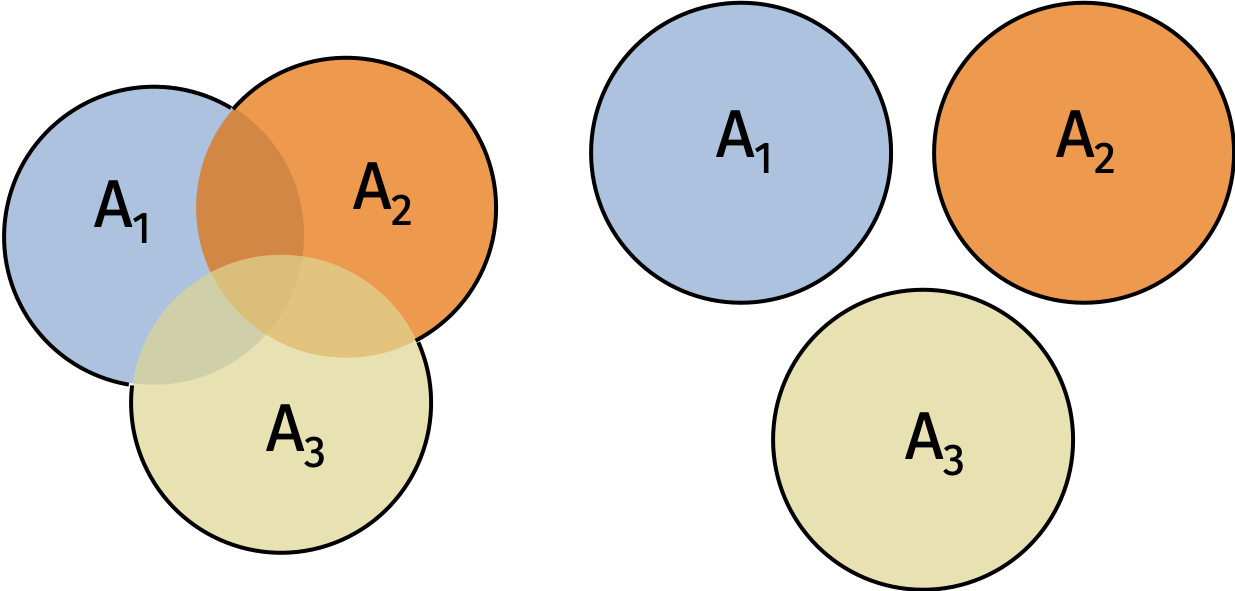
\includegraphics[width=.8\textwidth]{union_bound_proof.png}
	\end{center}
We will prove formally in a few slides.
\end{frame}

%\begin{frame}
%	\frametitle{proof of union bound}
%	\begin{lemma}[Union Bound]
%		For \emph{any} random events $A_1, \ldots, A_k$:
%		\begin{align*}
%			\Pr[A_1 \cup A_2 \cup \ldots \cup A_k] \leq \Pr[A_1] + \Pr[A_2] + \ldots +\Pr[A_k].
%		\end{align*}
%	\end{lemma}
%	Just use linearity of expectation!
%	\begin{align*}
%		\Pr[A_1 \cup A_2 \cup \ldots \cup A_k] &= \E[\max(\mathbbm{1}[A_1], \ldots, \mathbbm{1}[A_k])]\\
%		&\leq  \E[\mathbbm{1}[A_1] + \ldots + \mathbbm{1}[A_k]]\\
%		&= \E[\mathbbm{1}[A_1]] + \ldots + \E[\mathbbm{1}[A_k]]\\
%		& = \Pr[A_1] + \ldots +\Pr[A_k].
%	\end{align*}
%\end{frame}

\begin{frame}
	\frametitle{application of union bound}
	We want to prove that:
	\begin{align*}
		\Pr[\max_i s_i \geq C] = \Pr[(s_1 \geq C) \cup (s_2 \geq C) \cup \ldots \cup (s_n \geq C)] \leq \frac{1}{10}. 
	\end{align*}
	
	\alert{To do so, it suffices to prove that for all $i$:
		\begin{align*}
			\Pr[s_i \geq C] \leq \frac{1}{10n}. 
	\end{align*}}
	Why? Because then by the union bound, 
	\begin{align*}
		\Pr[\max_i s_i \geq C] &\leq \sum_{i=1}^n \Pr[s_i \geq C] \text{\hspace{1em}\blue{(Union bound)}}\\
		&\leq \sum_{i=1}^n \frac{1}{10n} = \frac{1}{10}. \qed
	\end{align*}
	

	\begin{block}{\vspace*{-3ex}}
		\small $n = $ number of balls and number of bins. $s_i$ is number of balls in bin $i$.
	\end{block}
\end{frame}

\begin{frame}
	\frametitle{new goal}
	Prove that for some $C$, 
	\begin{align*}
		\Pr[s_i \geq C] \leq \frac{1}{10n}. 
	\end{align*}
	
	\begin{center}
		This should look hard! We need to prove that $s_i < C$ (i.e. the $i^\text{th}$ bin has a small number of balls) with \emph{very high} probability (specifically $1- \frac{1}{10n})$. 
		
		\alert{\textbf{Markov's inequality is too weak of a bound for this.}}
	\end{center}
	
	\vspace{2em}
	\begin{block}{\vspace*{-3ex}}
		\small $n = $ number of balls and number of bins. $s_i$ is number of balls in bin $i$. $C =$ upper bound on maximum number of balls in any bin.
	\end{block}
\end{frame}


%\begin{frame}
%	\frametitle{attempt with markov's inequality}
%	\vspace{1em}
%	\textbf{Goal:} Prove that $\Pr[s_i \geq C] \leq \frac{1}{10n}$. 
%	\begin{itemize}
%		\item \textbf{Step 1.} Verify we can apply Markov's: $s_i$ takes on non-negative values only. Good to go!
%		\item \textbf{Step 2.} Apply Markov's: $\Pr[s_i \geq C] \leq \frac{\E[s_i]}{C} = \frac{1}{C}$. 
%	\end{itemize}
%	To prove our target statement, need to see $C = 10n$. 
%	
%	\emph{Meaningless!} There are only $n$ balls, so of course there can't be more than $10n$ in the most overloaded bin. 
%	
%	\vspace{2em}
%	\begin{block}{\vspace*{-3ex}}
%		\small $n = $ number of balls and number of bins. $s_i$ is number of balls in bin $i$. $\E[s_i] = 1$. $C =$ upper bound on maximum number of balls in any bin. \textbf{Markov's inequality}: for positive r.v. $X$, $\Pr[X \geq t] \leq \E[X]/t$.  
%	\end{block}
%\end{frame}

\begin{frame}
	\frametitle{application to balls into bins}
	\textbf{Goal:} Prove that $\Pr[s_i \geq C] \leq \frac{1}{10n}$. 
	\begin{itemize}
		\item \textbf{Step 1.} To apply Chebyshev's inequality, we need to understand $\sigma^2 = \Var[s_i]$. 
	\end{itemize}
	Use \emph{linearity of variance}. Let $s_{i,j}$ be a $\{0,1\}$ indicator random variable for the event that ball $j$ falls in bin $i$. We have:
	\begin{align*}
		s_i = \sum_{j=1}^n s_{i,j}. 
	\end{align*}
	And $s_{i,1}, \ldots, s_{i,n}$ are  independent so:
	\begin{align*}
		\Var[s_i] = \sum_{j=1}^n \Var[s_{i,j}]. 
	\end{align*}
	
	\vspace{0em}
	\begin{block}{\vspace*{-3ex}}
		\small $n = $ number of balls and number of bins. $s_i$ is number of balls in bin $i$. $\E[s_i] = 1$. $C =$ upper bound on max number of balls in bin. 
	\end{block}
\end{frame}

\begin{frame}
	\frametitle{variance analysis}

	\begin{align*}
		s_{i,j} = \begin{cases}
			1 \text{ with probability } \frac{1}{n}\\
			0 \text{ otherwise}.
		\end{cases}
	\end{align*}
	\begin{align*}
		\E[s_{i,j}] &= \hspace{10em}\\
		\E[s_{i,j}^2] &=  \hspace{10em}
	\end{align*}
	So:
	\begin{align*}
		\Var[s_{i,j}] = \E[s_{i,j}^2] - \E[s_{i,j}]^2 =  \hspace{10em}
	\end{align*}
	
	\vspace{0em}
	\begin{block}{\vspace*{-3ex}}
		\small $n = $ number of balls and number of bins. $s_{i,j}$ is event ball $j$ lands in bin $i$.
	\end{block}
\end{frame}

\begin{frame}
	\frametitle{applying chebyshev's}
	\textbf{Goal:} Prove that $\Pr[s_i \geq C] \leq \frac{1}{10n}$. 
	
	\textbf{Step 1.} To apply Chebyshev's inequality, we need to understand $\sigma^2 = \Var[s_i]$. 
	\begin{align*}
		\Var[s_i] = \sum_{j=1}^n \Var[s_{i,j}] = \sum_{j=1}^n \frac{1}{n} - \frac{1}{n^2} = {1- \frac{1}{n} \alert{\leq 1}.}
	\end{align*}
	
	\textbf{Step 2.} Apply Chebyshev's inequality:
	\begin{align*}
		&\Pr\left[\left|s_i - \E[s_i]\right| \geq k\cdot 1\right] \leq \frac{1}{k^2} \\
		&\text{which implies }\Pr\left[\left|s_i - 1\right| \geq k\cdot 1\right] \leq \frac{1}{k^2}.
	\end{align*}
	
	\vspace{0em}
	\begin{block}{\vspace*{-3ex}}
		\small $n = $ number of balls and number of bins. $s_i=$ number of balls in bin $i$.  $s_{i,j}$ is event ball $j$ lands in bin $i$. $\E[s_i] = 1$. 
	\end{block}
\end{frame}

\begin{frame}
	\frametitle{applying chebyshev's}
	\textbf{Goal:} Prove that $\Pr[s_i \geq C] \leq \frac{1}{10n}$. 
	
	We just proved: \blue{$\Pr[\left|s_i - 1\right| \geq k] \leq \frac{1}{k^2}$.}
	
	Setting $k = \sqrt{10n}$ gives: 
	\begin{align*}
		\Pr[\left|s_i - 1\right| &\geq \sqrt{10n}] \leq \frac{1}{10 n}.
	\end{align*}
	So, we have that:
	\begin{align*}
		\alert{\Pr[s_i \geq \sqrt{10n} + 1] \leq \frac{1}{10n}.}
	\end{align*}
	By the union bound argument from earlier, it thus holds that:
	\begin{align*}
		\Pr[\max_{i\in \{1,\ldots, n\}}s_i \geq \sqrt{10n} + 1] \leq \frac{1}{10}.
	\end{align*}
	
	
	\vspace{1em}
	\begin{block}{\vspace*{-3ex}}
		\small $n = $ number of balls and number of bins. $s_i$ is number of balls in bin $i$. $C =$ upper bound on maximum number of balls in any bin.
	\end{block}
\end{frame}

\begin{frame}
	\frametitle{final result}
	
	\begin{center}
		When hashing $n$ balls into $n$ bins, the maximum bin contains $o(\sqrt{n})$ balls with probability $\frac{9}{10}$.
		
		\vspace{1em}
		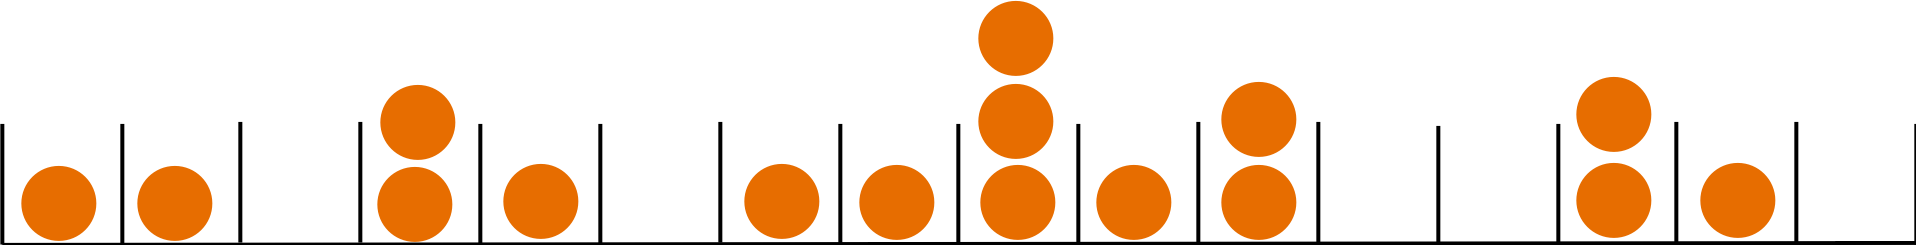
\includegraphics[width=.8\textwidth]{balls_into_bins.png}
		\vspace{1em}
		
		Much better than the trivial bound of $n$! 
	\end{center}
\end{frame}

\begin{frame}[t]
	\frametitle{proof a union bound}
	\begin{lemma}[Union Bound]
		For \emph{any} random events $A_1, \ldots, A_k$:
		\begin{align*}
			\Pr[A_1 \cup A_2 \cup \ldots \cup A_k] \leq \Pr[A_1] + \Pr[A_2] + \ldots +\Pr[A_k].
		\end{align*}
	\end{lemma}

		Let $X_i =  \mathbbm{1}[A_i]$ and apply Markov's to $S = \sum_{i=1}^k X_i$. 
	
\end{frame}

\begin{frame}
	\frametitle{takeaways}
	\textbf{Techniques used that will appear again:}
	\begin{itemize}
		\item Union bound to control the \emph{maximum} of many random variables. 
		\item Chebyshev's inequality to bound a variable whose variance we can compute.
		\item To compute the variance, break down random variable into smaller pieces and apply linearity of variance. 
	\end{itemize}
	
	\textbf{But...}
	For this problem we can actually use even stronger tools to prove a better bound of \emph{$O(\log n)$} for the most loaded bin.
	
\end{frame}



\begin{frame}
	\frametitle{beyond chebyshev}
	\textbf{Motivating question:} Is Chebyshev's Inequality tight?
	
	It is the worst case, but often not in reality.
	\vspace{-1em}
	\begin{figure}
		\centering
		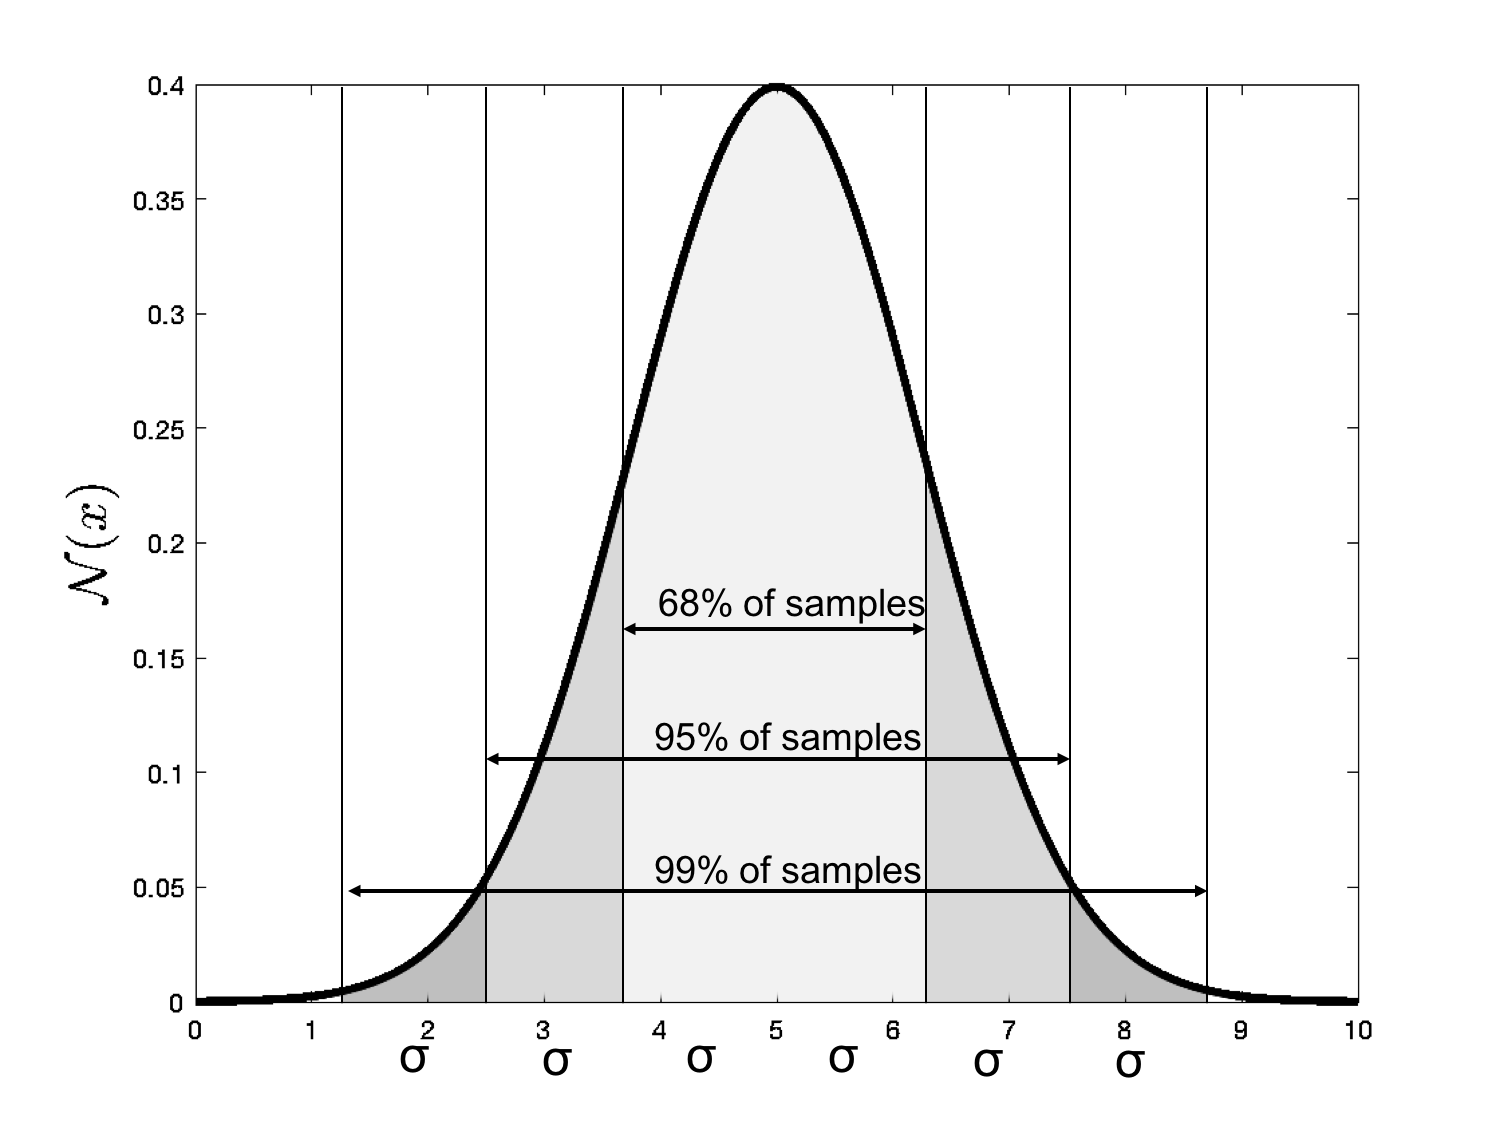
\includegraphics[width=0.4\textwidth]{689599rule.png}
			\vspace{-.5em}
		\caption{68-95-99 rule for Gaussian bell-curve. \alert{$\mathbf{X\sim N(0,\sigma^2)}$}}
	\end{figure}
			\vspace{-.5em}
	
	\begin{columns}
		\begin{column}{.5\textwidth}
			\small
			\textbf{Chebyshev's Inequality:}
			\vspace{-.5em}
			\begin{align*}
				\Pr\left(|X - \E[X]| \geq 1\sigma \right) &\leq 100\% \\
				\Pr\left(|X - \E[X]| \geq 2\sigma \right) &\leq 25\% \\
				\Pr\left(|X - \E[X]| \geq 3\sigma \right) &\leq 11\% \\
				\Pr\left(|X - \E[X]| \geq 4\sigma \right) &\leq 6\%.
			\end{align*}
		\end{column}
		\begin{column}{.5\textwidth}
			\small
			\textbf{Truth:}
			\vspace{-.5em}
			\begin{align*}
				\Pr\left(|X - \E[X]| \geq 1\sigma \right) &\approx 32\% \\
				\Pr\left(|X - \E[X]| \geq 2\sigma \right) &\approx 5\% \\
				\Pr\left(|X - \E[X]| \geq 3\sigma \right) &\approx 1\% \\
				\Pr\left(|X - \E[X]| \geq 4\sigma \right) &\approx .01\%
			\end{align*}
		\end{column}
	\end{columns}
\end{frame}

\begin{frame}
	\frametitle{gaussian concentration}
	\small
	For $X \sim \mathcal{N}(\mu,\sigma^2)$:
	\begin{align*}
		\Pr[X = \mu \pm x] \sim \frac{1}{\sigma\sqrt{2\pi}} \alert{\mathbf{e^{-x^2/2\sigma^2}}}
	\end{align*}
	\vspace{-1em}
	\begin{lemma}[Gaussian Tail Bound]
		For $X \sim \mathcal{N}(\mu,\sigma^2)$:\vspace{-.5em}
		\begin{align*}
			\Pr[|X - \E X| \geq k\cdot\sigma] \leq 2e^{-k^2/2}.
		\end{align*}
	\end{lemma}
	\begin{figure}
		\begin{subfigure}[t]{0.45\textwidth}
			\centering
			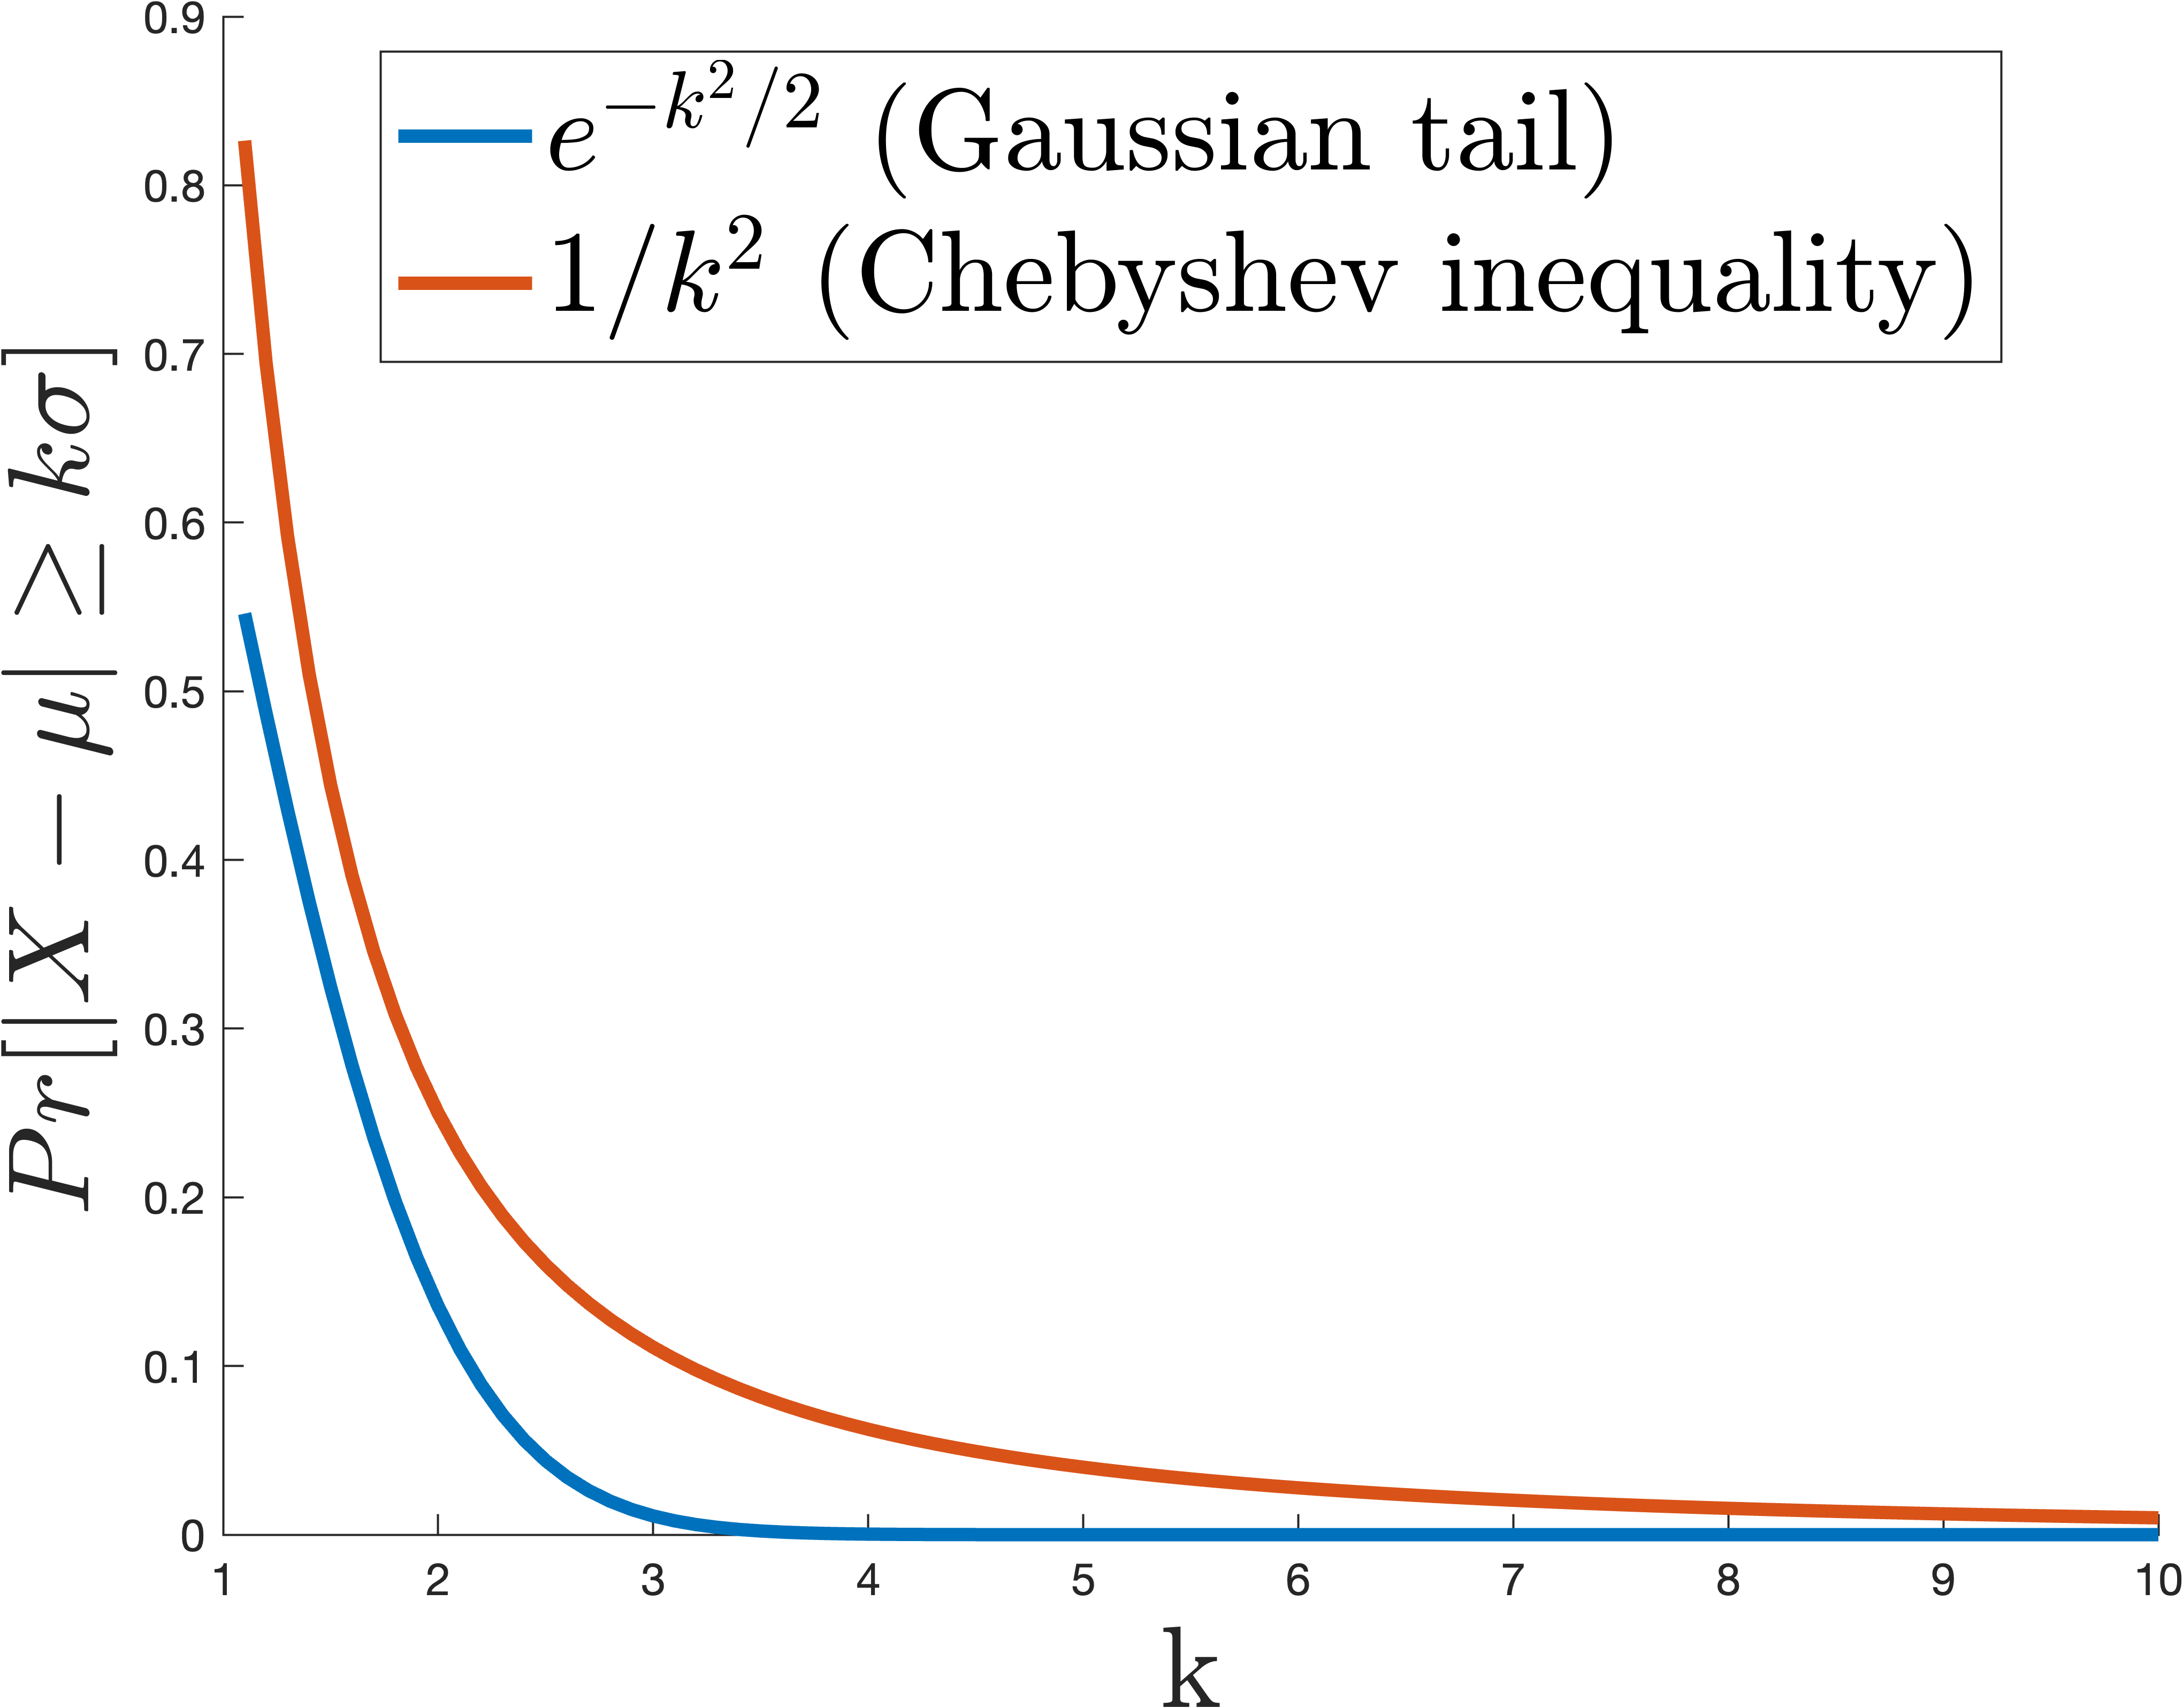
\includegraphics[width=\textwidth]{standardScale.png}
			\caption{Standard $y$-scale.}
		\end{subfigure}
		\hspace{1em}
		\begin{subfigure}[t]{0.45\textwidth}
			\centering
			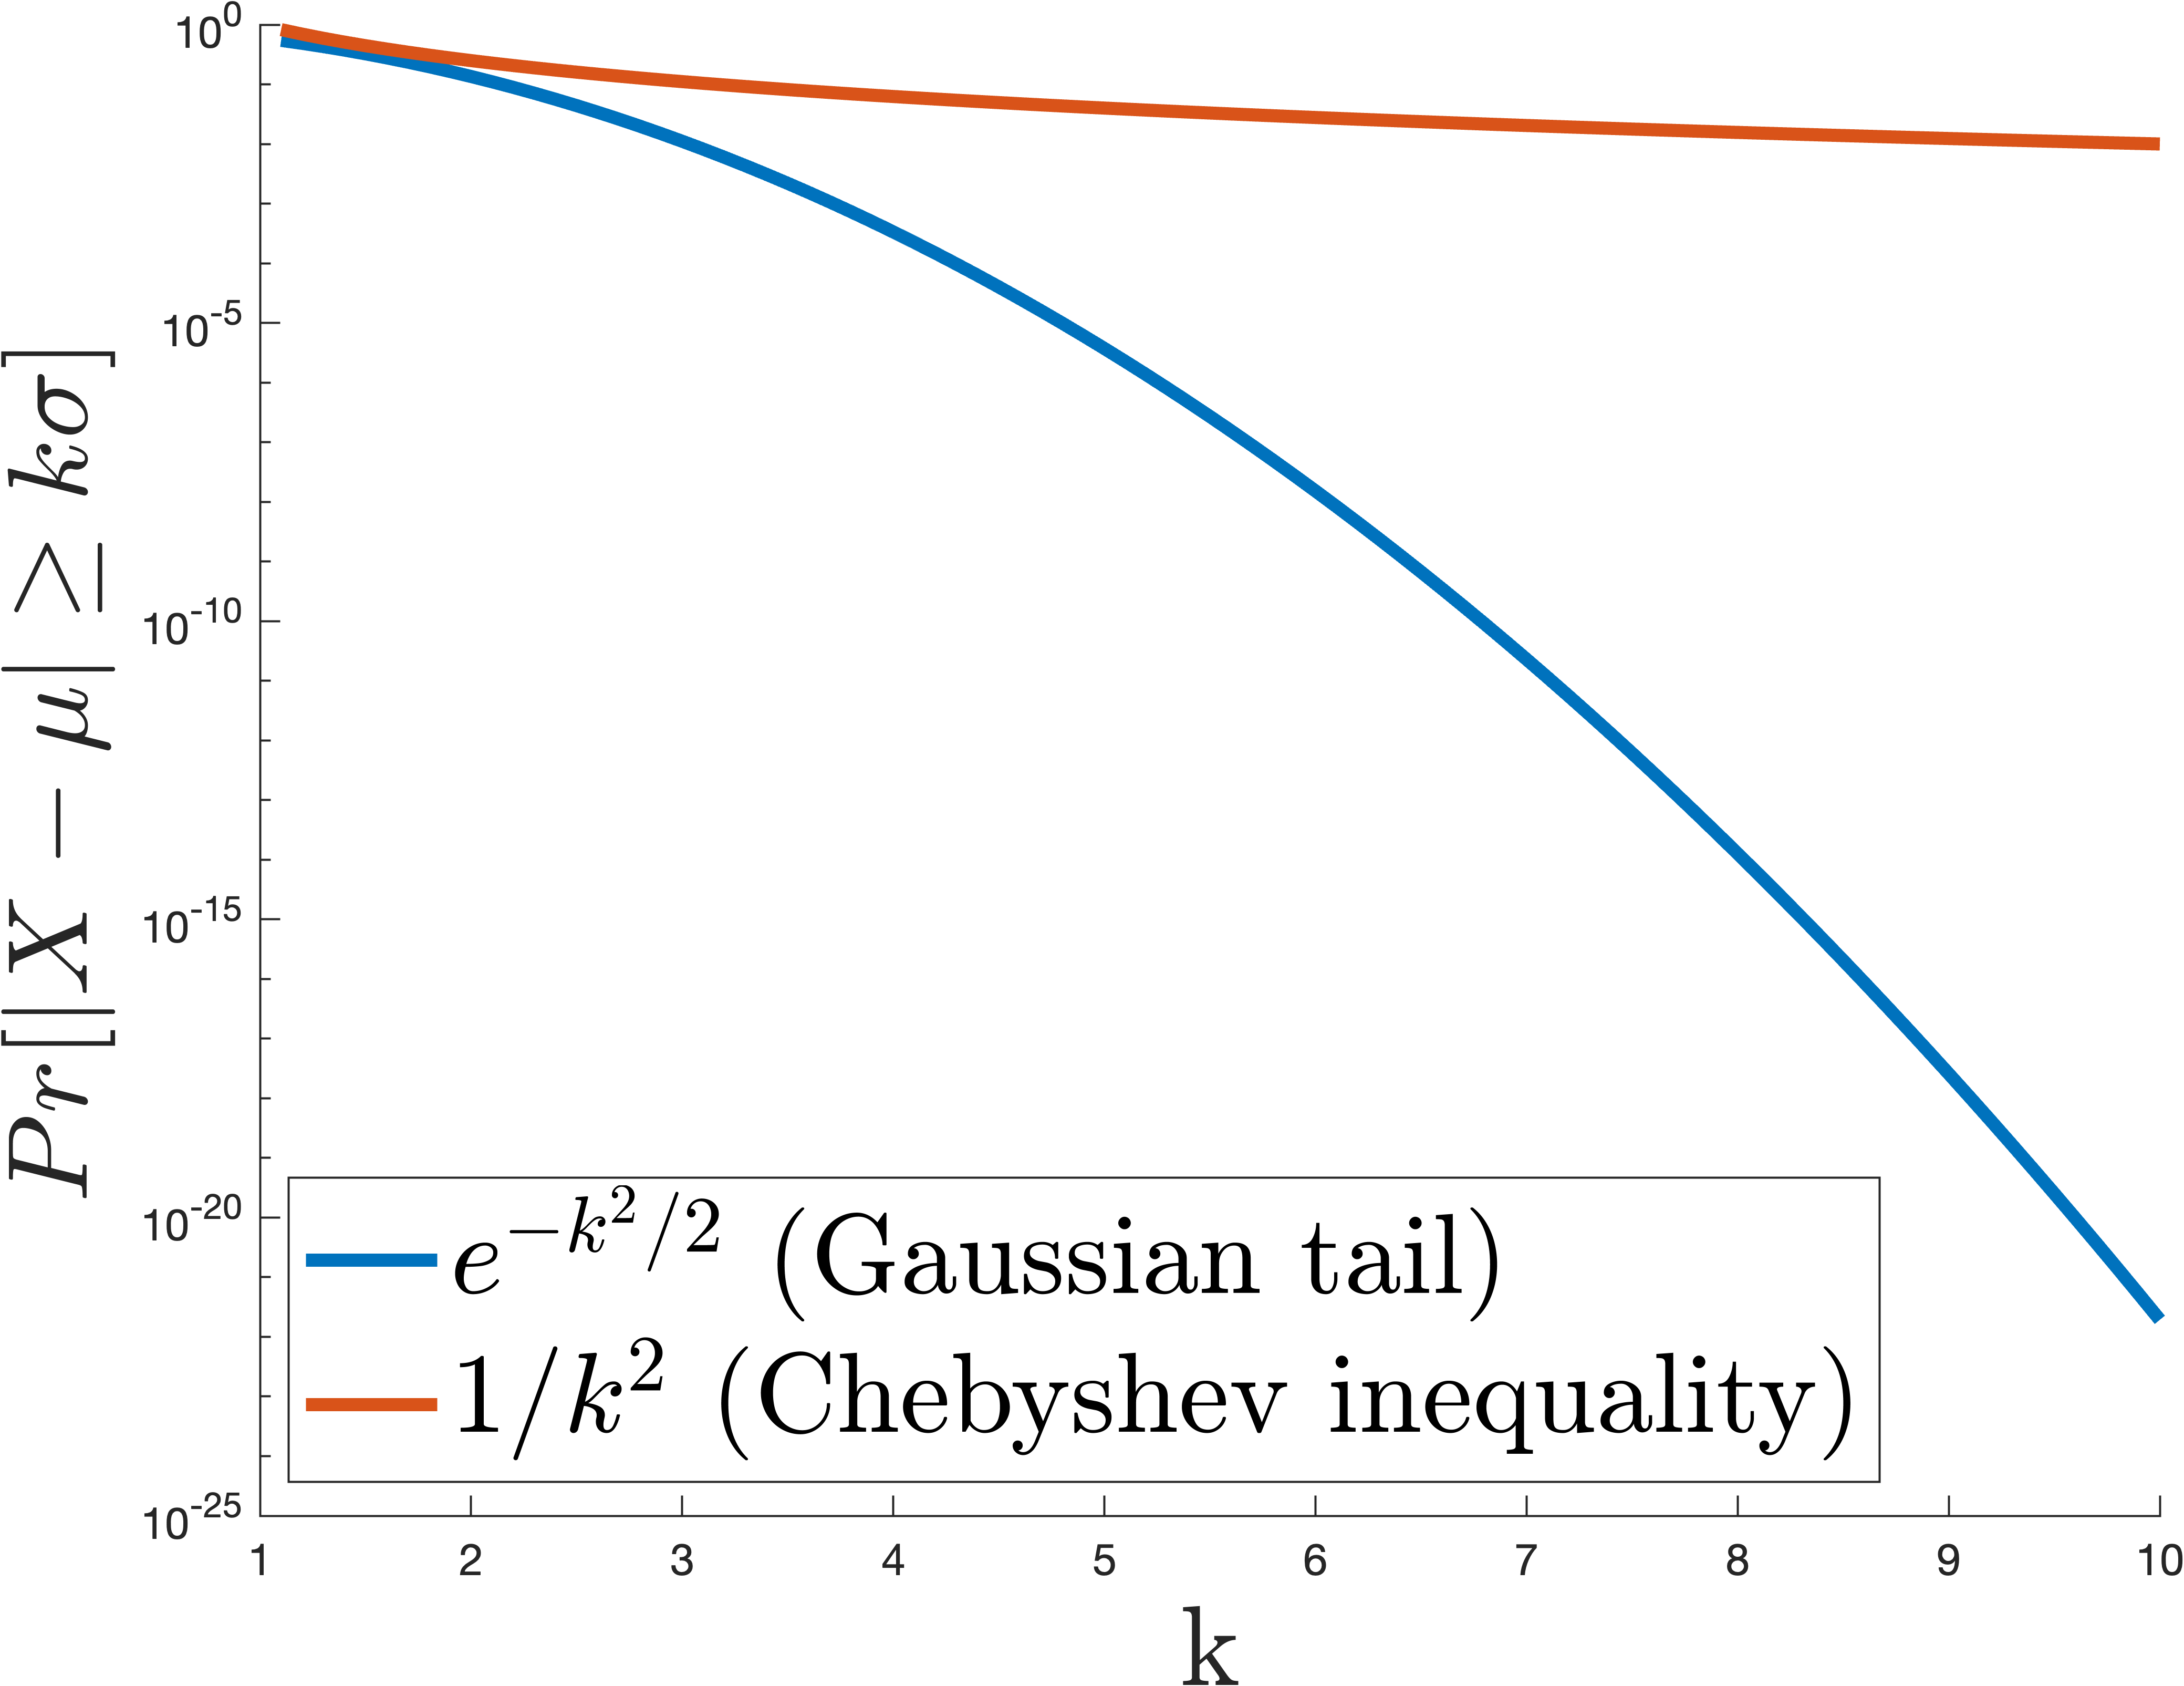
\includegraphics[width=\textwidth]{logScale.png}
			\caption{Logarithmic $y$-scale.}
		\end{subfigure}
	\end{figure}
	
\end{frame}

\begin{frame}
	\frametitle{gaussian concentration}
	\textbf{Takeaway:} Gaussian random variables concentrate much tighter around their expectation than variance alone (i.e. Chebyshevs's inequality)  predicts.
	
	\begin{center}
		\alert{\textbf{Why does this matter for algorithm design?}}
	\end{center}
\end{frame}

\begin{frame}
	\frametitle{central limit theorem}
	\begin{theorem}[CLT -- Informal]
		Any sum of \alert{mutually independent}, \alert{(identically distributed)}  r.v.'s $X_1,  \ldots, X_k$ with mean $\mu$ and finite variance $\sigma^2$ converges to a Gaussian r.v. with mean $k\cdot\mu$ and variance $k\cdot\sigma^2$, as $k\rightarrow \infty$.
		\vspace{-.5em}
		\begin{align*}
			S = \sum_{i=1}^n X_i \Longrightarrow \mathcal{N}(k\cdot\mu, k\cdot\sigma^2).
		\end{align*}	
		\vspace{-.5em}	
	\end{theorem}
	\vspace{-.5em}	
	\begin{figure}
		\begin{subfigure}[t]{0.4\textwidth}
			\centering
			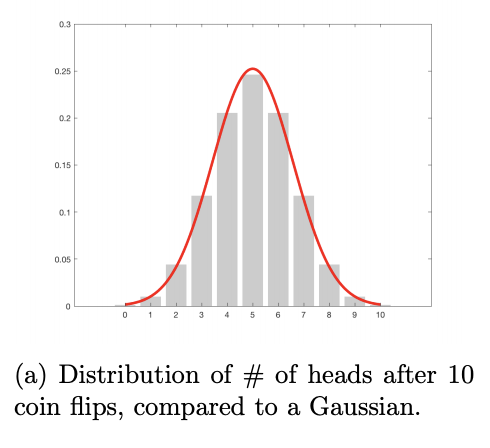
\includegraphics[width=\textwidth]{cltWide.png}
		\end{subfigure}
		\hspace{4em}
		\begin{subfigure}[t]{0.4\textwidth}
			\centering
			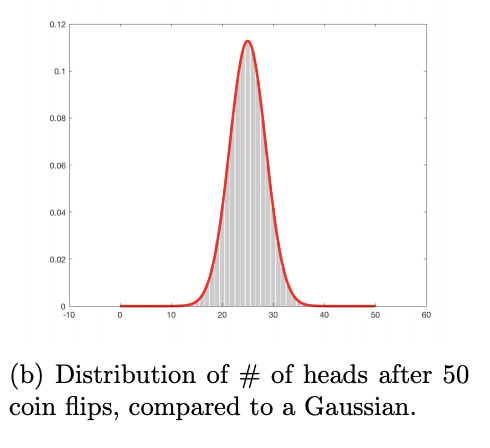
\includegraphics[width=\textwidth]{cltSkinny.png}
		\end{subfigure}
	\end{figure}
\end{frame}

\begin{frame}
	\frametitle{independence}
	Recall:
	\vspace{1em}
	\begin{definition}[Mutual Independence]
		Random variables $X_1, \ldots, X_k$ are \emph{mutually independent} if, for all possible values $v_1, \ldots, v_k$,
		\begin{align*}
			\Pr[X_1 = v_1, \ldots, X_k = v_k] = 	\Pr[X_1 = v_1]\cdot\ldots \cdot\Pr[X_k = v_k]
		\end{align*}
	\end{definition}
	\begin{center}
		\uncover<2->{\textbf{Strictly stronger than pairwise independence.}}
	\end{center}
\end{frame}

\begin{frame}
	\frametitle{exercise}
	\small 
	\begin{center}
	\textbf{If I flip a fair coin $100$ times, lower bound the chance I get between $30$ and $70$ heads?}
	\end{center}
	%	As in the previous lecture, we we would like to use concentration bounds to study the randomized load balancing problem. $n$ jobs are distributed randomly to $n$ servers using a hash function. Let $S_i$ be the number of jobs sent to server $i$. 
	%	\begin{enumerate}[label=(\alph*)]
	%		\item Using the CLT and our lemma for Gaussian concentration, estimate a bound for $\max_i[S_i]$. For example, your bound should take the form: $\Pr[max_i S_i \geq \alert{\textbf{B}}] \leq 1/10$. What's the smallest value of $\textbf{\alert{B}}$ you should hope to achieve? 
	%		\item Last class we proved the above bound with $\textbf{B} = O(\sqrt{n})$ using Chebyshev inequality. How does your bound compare?
	%	\end{enumerate}
	
	For this problem, we will assume the limit of the CLT holds \emph{exactly} -- i.e., that this sum looks exactly like a Gaussian random variable.
\begin{lemma}[Gaussian Tail Bound]
	For $X \sim \mathcal{N}(\mu,\sigma^2)$:\vspace{-.5em}
	\begin{align*}
		\Pr[|X - \E X| \geq k\cdot\sigma] \leq 2e^{-k^2/2}.
	\end{align*}
	\end{lemma}

$2e^{-8} = 06\%$
\end{frame}

%\begin{frame}
%	\frametitle{back-of-the-envelop calculation}
%	
\includegraphics[width=.9\textwidth]{envelope.jpg}
%\end{frame}


\begin{frame}
	\frametitle{quantitative versions of the clt}
	\textbf{These back-of-the-envelop calculations can be made rigorous!}
	\uncover<2->{\textbf{\alert{Lots of different ``versions'' of bound which do so.}}
		\begin{center}
			\begin{itemize}
				\item Chernoff bound
				\item Bernstein bound
				\item Hoeffding bound
				\item $\ldots$
			\end{itemize}
			Different assumptions on random varibles (e.g. binary vs. bounded), different forms (additive vs. multiplicative error), etc. \textbf{Wikipedia is your friend.}
		\end{center}
	}
\end{frame}

\begin{frame}
	\frametitle{quantitative versions of the clt}
	\begin{theorem}[Chernoff Bound]
		Let $X_1,X_2,\ldots,X_k$ be independent $\{0,1\}$-valued random variables and let
		$p_i = \E[X_i]$, where $0<p_i<1$.
		Then the sum $S = \sum_{i=1}^{k} X_i$, which has mean
		$\mu = \sum_{i=1}^{k} p_i$, satisfies
		\begin{align*}
			\Pr[S \geq (1+\epsilon)\mu] \leq e^{\frac{-\epsilon^2\mu}{2+ \epsilon}}.
		\end{align*}
		and for $0<\epsilon <1$
		\begin{align*}
			\Pr[S \leq (1-\epsilon)\mu] \leq e^{\frac{-\epsilon^2\mu}{2}}.
		\end{align*}
	\end{theorem} 
\end{frame}

\begin{frame}
	\frametitle{quantitative versions of the clt}
	\begin{theorem}[Bernstein Inequality]
		Let $X_1, X_2, \ldots, X_k$ be independent random variables with each $X_i \in [-1,1]$.
		Let $\mu_i =\E[X_i]$ and $\sigma_i^2 = \Var[X_i]$. Let  $\mu =\sum_i \mu_i$ and $\sigma^2 =\sum_i \sigma_i^2$. Then, for $k \leq \frac{1}{2}\sigma$, $S =\sum_i X_i$ satisfies
		$$\Pr[|S - \mu| > k\cdot \sigma] \leq  2 e^{-\frac{k^2}{4}}.$$
	\end{theorem}
\end{frame}

\begin{frame}
	\frametitle{quantitative versions of the clt}
	\begin{theorem}[Hoeffding Inequality]
		Let $X_1, X_2, \ldots, X_k$ be independent random variables with each $X_i \in [a_i,b_i]$.
		Let $\mu_i =\E[X_i]$ and $\mu =\sum_i \mu_i$. Then, for any $\alpha > 0$, $S =\sum_i X_i$ satisfies:
		$$\Pr[|S - \mu| > \alpha] \leq  2 e^{-\frac{\alpha^2}{\sum_{i=1}^k (b_i-a_i)^2}}.$$
	\end{theorem}
\end{frame}

\begin{frame}
	\frametitle{how are these bounds proven?}
	Variance is a natural \emph{measure of central tendency}, but there are others. 
	\begin{align*}
		q^\text{th} \text{ central moment: } \E[(X-\E X)^q]
	\end{align*}
	$k = 2$ gives the variance. Proof of Chebyshev's applies Markov's inequality to the random variable $(X - \E X)^2)$.
	
	\textbf{Idea in brief:} Apply Markov's inequality to $\E[(X-\E X)^q$ for larger $q$, or more generally to $f(X-\E X)$ for some other non-negative function $f$. E.g., to $\exp(X-\E X)$. 
\end{frame}

\begin{frame}
	\frametitle{chernoff bound application}
	\small
	\textbf{Sample Application:} Flip biased coin $k$ times: i.e. the coin is heads with probability $b$. As long as $k \geq O\left(\frac{\log(1/\delta)}{\epsilon^2}\right)$,
	\vspace{-.5em}
	\begin{align*}
		\Pr[|\text{\# heads} - b\cdot k| \geq \epsilon k] \leq \delta 
	\end{align*}
	
	\textbf{Setup:}
	Let $X_i = \mathbbm{1}[i^\text{th} \text{ flip is heads}]$. Want bound probability that  $\sum_{i=1}^k X_i$ deviates from it's expectation.
	
	\textbf{Corollary of Chernoff bound}: Let $S = \sum_{i=1}^k X_i$ and $\mu = \E[S]$. For $0< \epsilon < 1$, 
	\vspace{-.75em}
	\begin{align*}
		\Pr[|S - \mu| \geq \epsilon \mu] \leq 2e^{-\epsilon^2 \mu/3}
	\end{align*} 
	\vspace{6em}
\end{frame}

\begin{frame}
	\frametitle{chernoff bound application}
	\textbf{Sample Application:} Flip biased coin $k$ times: i.e. the coin is heads with probability $b$. As long as $k \geq O\left(\frac{\log(1/\delta)}{\epsilon^2}\right)$,
	\begin{align*}
		\Pr[|\text{\# heads} - b\cdot k| \geq \epsilon k] \leq \delta 
	\end{align*}
	
	
	
	Pay very little for higher probability -- if you increase the number of coin flips by 4x, $\delta$ goes from $1/10 \rightarrow 1/100 \rightarrow 1/10000$
\end{frame}

%\begin{frame}
%	\frametitle{application to minhash}
%	Let $J = J(\bv{q},\bv{y})$ denote the true Jaccard similarity.
%	
%	\textbf{Estimator:} $\tilde{J} = \frac{1}{k} \sum_{i=1}^k \mathbbm{1}[c_i(\bv{q}) = c_i(\bv{y})]$. 
%	
%	By the analysis above,
%	\begin{align*}
%		\Pr[|\tilde{J} - J| \geq \epsilon] = \Pr[|\tilde{J} \cdot k - J\cdot k| \geq \epsilon k] \leq \delta 
%	\end{align*} 
%	as long as $k = O\left(\frac{\log(1/\delta)}{\epsilon^2}\right)$. 
%	
%	Much better than the $k = O\left(\frac{1}{\delta\epsilon^2}\right)$.
%	
%	For example, if we had a data base of $n=1,000,000$ songs, setting $\delta = \frac{1}{n}$ would only require space depending on $\log(n) \approx 14$, instead of on $n=1,000,000$.  
%	
%\end{frame}


\begin{frame}
	\frametitle{load balancing}
	\small
	We are going to see a more interesting application of exponential concentration bounds to the randomized load balancing problem. $n$ jobs are distributed randomly to $n$ servers using a hash function. Let $S_i$ be the number of jobs sent to server $i$.  What's the smallest $\alert{\mathbf{B}}$ for which we can prove:
	\begin{align*}
		\Pr[\max_i S_i \geq \alert{\mathbf{B}}] \leq 1/10
	\end{align*}
	\vspace{-1em}
	\begin{center}
		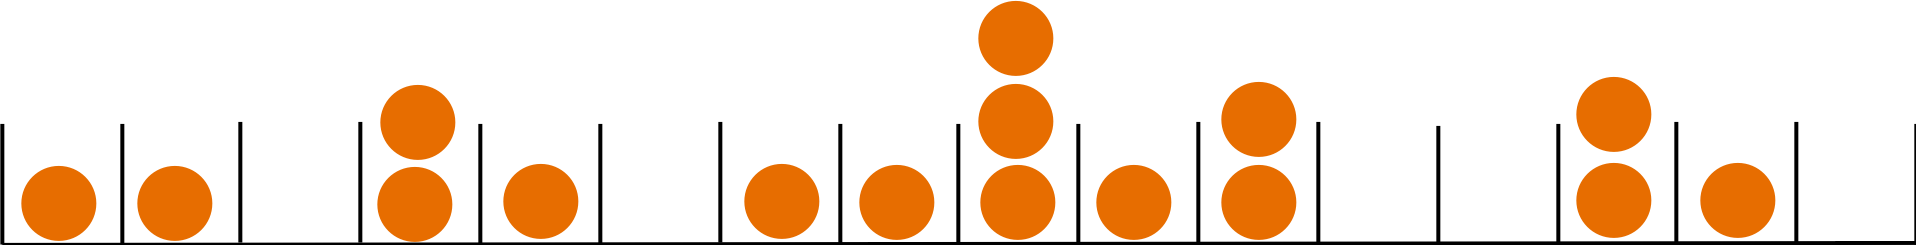
\includegraphics[width=.6\textwidth]{ballsinbins.png}
	\end{center}
	
	\textbf{Recall:} Suffices to prove that, for any $i$, $\Pr[ S_i \geq {\mathbf{B}}] \leq 1/10n$:
	\begin{align*}
		\Pr[\max_i S_i \geq {\mathbf{B}}] &= \Pr[S_1 \geq {\mathbf{B}} \text{ or } \ldots \text{ or } S_1 \geq {\mathbf{B}}] \\
		&\leq \Pr[S_1 \geq {\mathbf{B}}] + \ldots + \Pr[S_n \geq {\mathbf{B}}] \text{\hspace{1em} (union bound)}.
	\end{align*}
\end{frame}

\begin{frame}[t]
	\frametitle{load balancing}
	\begin{theorem}[Chernoff Bound]
		Let $X_1,X_2,\ldots,X_n$ be independent $\{0,1\}$-valued random variables and let
		$p_i = \E[X_i]$, where $0<p_i<1$.
		Then the sum $S = \sum_{j=1}^{n} X_i$, which has mean
		$\mu = \sum_{j=1}^{n} p_i$, satisfies
		\begin{align*}
			\Pr[X \geq (1+\epsilon)\mu] \leq e^{\frac{-\epsilon^2\mu}{2+ \epsilon}}.
		\end{align*}
	\end{theorem} 
	Consider a single bin. Let $X_j = \mathbbm{1}[\text{ball $j$ lands in that bin}]$. $\E[X_j] = \frac{1}{n}$. $S = \sum_{j=1}^n X_j$, so $\mu = 1$. 
	\begin{align*}
		\Pr[S \geq (1+c\log n)\mu] \leq e^{\frac{-c^2\log^2 n}{2 + c\log n}} \leq e^{\frac{-c\log^2 n}{2\log n}} \leq e^{-.5c\log n} \leq \frac{1}{10n},
	\end{align*}
	for sufficiently large $c$
	
\end{frame}

\begin{frame}
	\frametitle{power of two choices}
	\begin{center}\alert{\textbf{So max load for randomized load balancing is $O(\log n)$!}} Best we could prove with Chebyshev's was $O(\sqrt{n})$. \end{center}
\end{frame}

\begin{frame}
	\frametitle{power of two choices}
	\textbf{Power of 2 Choices:} Instead of assigning job to random server, choose 2 random servers and assign to the least loaded. With probability $1/10$ the maximum load is bounded by:
	
	(a) $O(\log n)$ \hspace{1em} (b) $O(\sqrt{\log n})$  \hspace{1em}  (c) $O(\log \log n)$  \hspace{1em} (d) $O(1)$
	\begin{center}
		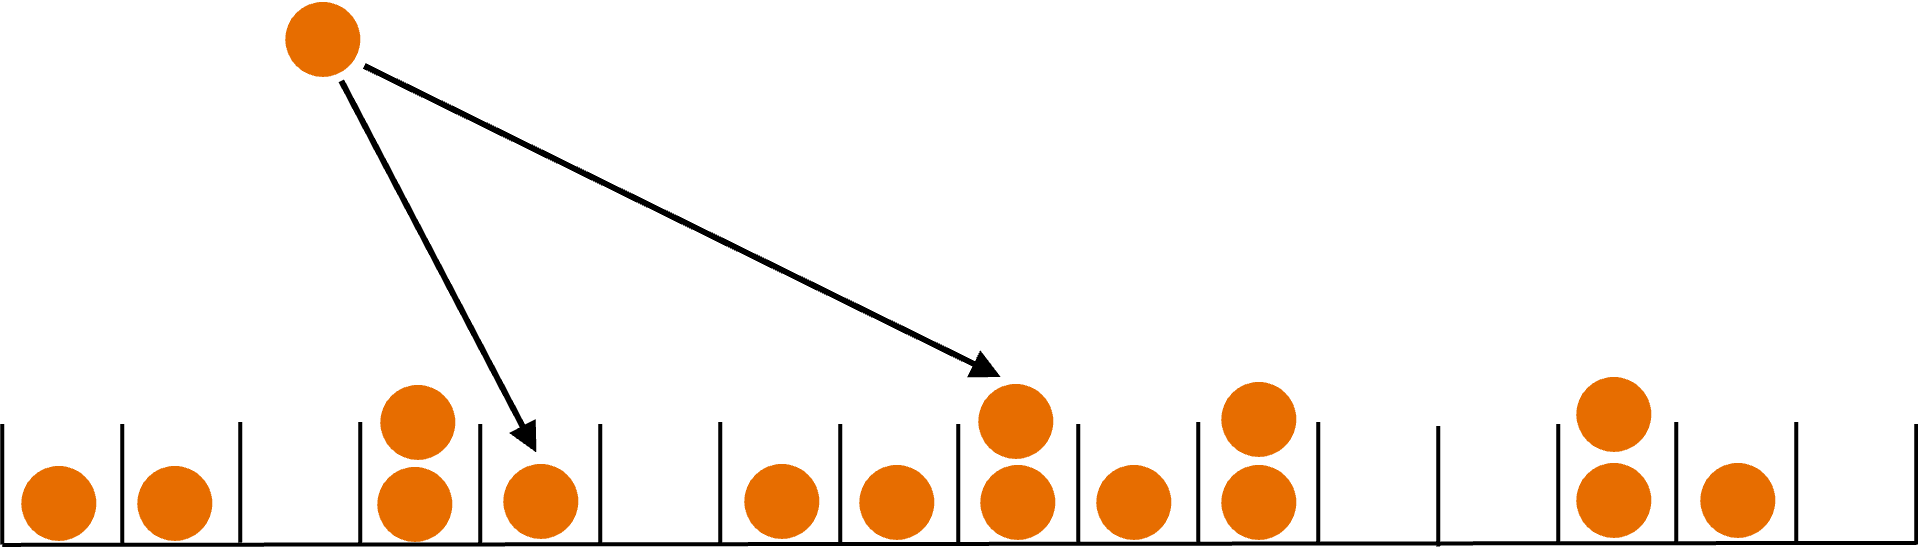
\includegraphics[width=.9\textwidth]{power_of_two.png}
	\end{center}
\end{frame}

\end{document} 








